%% For double-blind review submission, w/o CCS and ACM Reference (max submission space)
\documentclass[sigplan,10pt,review,anonymous,nonacm]{acmart}
\settopmatter{printfolios=true,printccs=false,printacmref=false}
%% For double-blind review submission, w/ CCS and ACM Reference
%\documentclass[sigplan,review,anonymous]{acmart}\settopmatter{printfolios=true}
%% For single-blind review submission, w/o CCS and ACM Reference (max submission space)
%\documentclass[sigplan,review]{acmart}\settopmatter{printfolios=true,printccs=false,printacmref=false}
%% For single-blind review submission, w/ CCS and ACM Reference
%\documentclass[sigplan,review]{acmart}\settopmatter{printfolios=true}
%% For final camera-ready submission, w/ required CCS and ACM Reference
%\documentclass[sigplan]{acmart}\settopmatter{}


%% Conference information
%% Supplied to authors by publisher for camera-ready submission;
%% use defaults for review submission.
\acmConference[PL'18]{ACM SIGPLAN Conference on Programming Languages}{January 01--03, 2018}{New York, NY, USA}
\acmYear{2018}
\acmISBN{} % \acmISBN{978-x-xxxx-xxxx-x/YY/MM}
\acmDOI{} % \acmDOI{10.1145/nnnnnnn.nnnnnnn}
\startPage{1}

%% Copyright information
%% Supplied to authors (based on authors' rights management selection;
%% see authors.acm.org) by publisher for camera-ready submission;
%% use 'none' for review submission.
\setcopyright{none}
%\setcopyright{acmcopyright}
%\setcopyright{acmlicensed}
%\setcopyright{rightsretained}
%\copyrightyear{2018}           %% If different from \acmYear

%% Bibliography style
\bibliographystyle{ACM-Reference-Format}
%% Citation style
%\citestyle{acmauthoryear}  %% For author/year citations
%\citestyle{acmnumeric}     %% For numeric citations
%\setcitestyle{nosort}      %% With 'acmnumeric', to disable automatic
                            %% sorting of references within a single citation;
                            %% e.g., \cite{Smith99,Carpenter05,Baker12}
                            %% rendered as [14,5,2] rather than [2,5,14].
%\setcitesyle{nocompress}   %% With 'acmnumeric', to disable automatic
                            %% compression of sequential references within a
                            %% single citation;
                            %% e.g., \cite{Baker12,Baker14,Baker16}
                            %% rendered as [2,3,4] rather than [2-4].


%%%%%%%%%%%%%%%%%%%%%%%%%%%%%%%%%%%%%%%%%%%%%%%%%%%%%%%%%%%%%%%%%%%%%%
%% Note: Authors migrating a paper from traditional SIGPLAN
%% proceedings format to PACMPL format must update the
%% '\documentclass' and topmatter commands above; see
%% 'acmart-pacmpl-template.tex'.
%%%%%%%%%%%%%%%%%%%%%%%%%%%%%%%%%%%%%%%%%%%%%%%%%%%%%%%%%%%%%%%%%%%%%%


%% Some recommended packages.
\usepackage{booktabs}   %% For formal tables:
                        %% http://ctan.org/pkg/booktabs
\usepackage{subcaption} %% For complex figures with subfigures/subcaptions
                        %% http://ctan.org/pkg/subcaption


\usepackage[T1]{fontenc} % fix missing font cmtt
\usepackage{amsmath}
\let\Bbbk\relax
\usepackage{amssymb} % Vdash
\usepackage{graphicx} % rotatebox
\usepackage{stmaryrd} % llparenthesis
\usepackage{anyfontsize} % workaround for font size difference warning
\usepackage{todonotes}
\usepackage{listings}
\usepackage{tikz}
\usetikzlibrary{calc,fit,tikzmark,plotmarks,arrows.meta,positioning,overlay-beamer-styles}

\usepackage{cancel} % slash over symbol
\usepackage{hyperref}
\renewcommand\UrlFont{\color{blue}\rmfamily}
\def\figureautorefname{Fig.}
\def\lemmaautorefname{Lemma}
\let\subsectionautorefname\sectionautorefname
\let\subsubsectionautorefname\sectionautorefname
\newcommand{\rulesref}[1]{Rules (\ref{#1})}
\newcommand{\ruleref}[1]{Rule (\ref{#1})}

\usepackage{xcolor}
\definecolor{hazelgreen}{RGB}{7,63,36}
\definecolor{hazellightgreen}{RGB}{103,138,97}
\definecolor{hazelyellow}{RGB}{245,222,179}
\definecolor{hazellightyellow}{RGB}{254,254,234}

\newcommand{\highlight}[1]{\colorbox{yellow}{$\displaystyle #1$}}

%% Joshua Dunfield macros
\def\OPTIONConf{1}
\usepackage{jdunfield}
\usepackage{rulelinks} % hyperlink of rule name
% \usepackage{pfsteps}
\makeatletter
\newcommand{\savelocalsteps}[1]{
  \@ifundefined{c@#1}
    {% the counter doesn't exist
     \newcounter{#1}
   }{}
  \setcounter{#1}{\value{pfsteps@pfc@local}}
}
\makeatother
\newcommand{\restorelocalsteps}[1]{\setcounter{pfsteps@pfc@local}{\value{#1}}}

% !TEX root = ./patterns-paper.tex

% reverse Vdash
\newcommand{\dashV}{\mathbin{\rotatebox[origin=c]{180}{$\Vdash$}}}

% Violet hotdogs; highlight color helps distinguish them
\newcommand{\llparenthesiscolor}{\textcolor{violet}{\llparenthesis}}
\newcommand{\rrparenthesiscolor}{\textcolor{violet}{\rrparenthesis}}

% HTyp and HExp
\newcommand{\hcomplete}[1]{#1~\mathsf{complete}}

% HTyp
\newcommand{\htau}{\dot{\tau}}
\newcommand{\tarr}[2]{\inparens{#1 \rightarrow #2}}
\newcommand{\tarrnp}[2]{#1 \rightarrow #2}
\newcommand{\trul}[2]{\inparens{#1 \Rightarrow #2}}
\newcommand{\tnum}{\mathtt{num}}
\newcommand{\tehole}{\llparenthesiscolor\rrparenthesiscolor}
\newcommand{\tsum}[2]{\inparens{{#1} + {#2}}}
\newcommand{\tprod}[2]{\inparens{{#1} \times {#2}}}
\newcommand{\tunit}{\mathtt{1}}
\newcommand{\tvoid}{\mathtt{0}}

\newcommand{\tcompat}[2]{#1 \sim #2}
\newcommand{\tincompat}[2]{#1 \nsim #2}

% HExp
\newcommand{\hexp}{\dot{e}}
\newcommand{\hlam}[3]{\inparens{\lambda #1:#2.#3}}
\newcommand{\hap}[2]{#1(#2)}
\newcommand{\hapP}[2]{(#1)~(#2)} % Extra paren around function term
\newcommand{\hnum}[1]{\underline{#1}}
\newcommand{\hadd}[2]{\inparens{#1 + #2}}
\newcommand{\hpair}[2]{\inparens{#1 , #2}}
\newcommand{\htriv}{()}
\newcommand{\hehole}{\llparenthesiscolor\rrparenthesiscolor}
\newcommand{\hhole}[1]{\llparenthesiscolor#1\rrparenthesiscolor}
\newcommand{\hindet}[1]{\lceil#1\rceil}
\newcommand{\hinj}[2]{\mathtt{inj}_{#1}({#2})}
\newcommand{\hinl}[2]{\mathtt{inl}_{#1}({#2})}
\newcommand{\hinr}[2]{\mathtt{inr}_{#1}({#2})}
\newcommand{\hinlp}[1]{\mathtt{inl}(#1)}
\newcommand{\hinrp}[1]{\mathtt{inr}(#1)}
\newcommand{\hmatch}[2]{\mathtt{match}(#1) \{#2\}}
\newcommand{\hcase}[5]{\mathtt{case}({#1},{#2}.{#3},{#4}.{#5})}
\newcommand{\hrules}[2]{\inparens{#1 \mid #2}}
\newcommand{\hrul}[2]{#1 \Rightarrow #2}

\newcommand{\hGamma}{\dot{\Gamma}}
\newcommand{\domof}[1]{\text{dom}(#1)}
\newcommand{\hsyn}[3]{#1 \vdash #2 \Rightarrow #3}
\newcommand{\hana}[3]{#1 \vdash #2 \Leftarrow #3}
\newcommand{\hexptyp}[3]{#1 \vdash #2 : #3}
\newcommand{\hpattyp}[3]{#1 : #2 \dashV #3}
\newcommand{\hpatmatch}[3]{#1 \vartriangleright #2 \dashV #3}
\newcommand{\hval}[1]{#1 ~\mathtt{val}}
\newcommand{\herr}[1]{#1 ~\mathtt{err}}

% ZTyp and ZExp
\newcommand{\zlsel}[1]{{\bowtie}{#1}}
\newcommand{\zrsel}[1]{{#1}{\bowtie}}
\newcommand{\zwsel}[1]{
  \setlength{\fboxsep}{0pt}
  \colorbox{green!10!white!100}{
    \ensuremath{{{\textcolor{Green}{{\hspace{-2px}\triangleright}}}}{#1}{\textcolor{Green}{\triangleleft{\vphantom{\tehole}}}}}}
}

\newcommand{\removeSel}[1]{#1^{\diamond}}

% ZTyp
\newcommand{\ztau}{\hat{\tau}}

% ZExp
\newcommand{\zexp}{\hat{e}}

% Direction
\newcommand{\dParent}{\mathtt{parent}}
\newcommand{\dChildn}[1]{\mathtt{child}~\mathtt{{#1}}}
\newcommand{\dChildnm}[1]{\mathtt{child}~{#1}}

% Action
\newcommand{\aMove}[1]{\mathtt{move}~#1}
	\newcommand{\zrightmost}[1]{\mathsf{rightmost}(#1)}
	\newcommand{\zleftmost}[1]{\mathsf{leftmost}(#1)}
\newcommand{\aSelect}[1]{\mathtt{sel}~#1}
\newcommand{\aDel}{\mathtt{del}}
\newcommand{\aReplace}[1]{\mathtt{replace}~#1}
\newcommand{\aConstruct}[1]{\mathtt{construct}~#1}
\newcommand{\aConstructx}[1]{#1}
\newcommand{\aFinish}{\mathtt{finish}}

\newcommand{\performAna}[5]{#1 \vdash #2 \xlongrightarrow{#4} #5 \Leftarrow #3}
\newcommand{\performAnaI}[5]{#1 \vdash #2 \xlongrightarrow{#4}\hspace{-3px}{}^{*}~ #5 \Leftarrow #3}
\newcommand{\performSyn}[6]{#1 \vdash #2 \Rightarrow #3 \xlongrightarrow{#4} #5 \Rightarrow #6}
\newcommand{\performSynI}[6]{#1 \vdash #2 \Rightarrow #3 \xlongrightarrow{#4}\hspace{-3px}{}^{*}~ #5 \Rightarrow #6}
\newcommand{\performTyp}[3]{#1 \xlongrightarrow{#2} #3}
\newcommand{\performTypI}[3]{#1 \xlongrightarrow{#2}\hspace{-3px}{}^{*}~#3}

\newcommand{\performMove}[3]{#1 \xlongrightarrow{#2} #3}
\newcommand{\performDel}[2]{#1 \xlongrightarrow{\aDel} #2}

% Form
\newcommand{\farr}{\mathtt{arrow}}
\newcommand{\fnum}{\mathtt{num}}
\newcommand{\fsum}{\mathtt{sum}}

\newcommand{\fasc}{\mathtt{asc}}
\newcommand{\fvar}[1]{\mathtt{var}~#1}
\newcommand{\flam}[1]{\mathtt{lam}~#1}
\newcommand{\fap}{\mathtt{ap}}
% \newcommand{\farg}{\mathtt{arg}}
\newcommand{\fnumlit}[1]{\mathtt{lit}~#1}
\newcommand{\fplus}{\mathtt{plus}}
\newcommand{\fhole}{\mathtt{hole}}
\newcommand{\fnehole}{\mathtt{nehole}}

\newcommand{\finj}[1]{\mathtt{inj}~#1}
\newcommand{\fcase}[2]{\mathtt{case}~#1~#2}

% Talk about formal rules in example
\newcommand{\refrule}[1]{\textrm{Rule~(#1)}}

\newcommand{\herase}[1]{\left|#1\right|_\textsf{erase}}

\newcommand{\arrmatch}[2]{#1 \blacktriangleright_{\rightarrow} #2}


\newcommand{\TABperformAna}[5]{#1 \vdash & #2                & \xlongrightarrow{#4} & #5 & \Leftarrow #3}
\newcommand{\TABperformSyn}[6]{#1 \vdash & #2 \Rightarrow #3 & \xlongrightarrow{#4} & #5 \Rightarrow #6}
\newcommand{\TABperformTyp}[3]{& #1 & \xlongrightarrow{#2} & #3}

\newcommand{\TABperformMove}[3]{#1 & \xlongrightarrow{#2} & #3}
\newcommand{\TABperformDel}[2]{#1 \xlongrightarrow{\aDel} #2}

\newcommand{\sumhasmatched}[2]{#1 \mathrel{\textcolor{black}{\blacktriangleright_{+}}} #2}

\newcommand{\subminsyn}[1]{\mathsf{submin}_{\Rightarrow}(#1)}
\newcommand{\subminana}[1]{\mathsf{submin}_{\Leftarrow}(#1)}


\newcommand{\inparens}[1]{{\color{gray}(}#1{\color{gray})}}

%% rule names for appendix
\newcommand{\rname}[1]{\textsc{#1}}
\newcommand{\gap}{\vspace{7pt}}


% !TEX root = pattern-paper.tex
%% Statics

% typing of internal expressions
\newrulecommand{TVar}{TVar}
\newrulecommand{TNum}{TNum}
\newrulecommand{TLam}{TLam}
\newrulecommand{TAp}{TAp}
\newrulecommand{TPair}{TPair}
\newrulecommand{TPrl}{TPrl}
\newrulecommand{TPrr}{TPrr}
\newrulecommand{TInl}{TInl}
\newrulecommand{TInr}{TInr}
\newrulecommand{TMatchZPre}{TMatchZPre}
\newrulecommand{TMatchNZPre}{TMatchNZPre}
\newrulecommand{TEHole}{TEHole}
\newrulecommand{THole}{THole}

% typing of rule and rules
\newrulecommand{TRule}{TRule}
\newrulecommand{TOneRules}{TOneRules}
\newrulecommand{TRules}{TRules}

% typing of pattern
\newrulecommand{PTVar}{PTVar}
\newrulecommand{PTNum}{PTNum}
\newrulecommand{PTWild}{PTWild}
\newrulecommand{PTPair}{PTPair}
\newrulecommand{PTInl}{PTInl}
\newrulecommand{PTInr}{PTInr}
\newrulecommand{PTEHole}{PTEHole}
\newrulecommand{PTHole}{PTHole}

%% Dynamics

% typing of substitution
\newrulecommand{STEmpty}{STEmpty}
\newrulecommand{STExtend}{STExtend}

% refutable pattern
\newrulecommand{RNum}{RNum}
\newrulecommand{REHole}{REHole}
\newrulecommand{RHole}{RHole}
\newrulecommand{RInl}{RInl}
\newrulecommand{RInr}{RInr}
\newrulecommand{RPairL}{RPairL}
\newrulecommand{RPairR}{RPairR}

% match
\newrulecommand{MVar}{MVar}
\newrulecommand{MNum}{MNum}
\newrulecommand{MWild}{MWild}
\newrulecommand{MPair}{MPair}
\newrulecommand{MEHolePair}{MEHolePair}
\newrulecommand{MHolePair}{MHolePair}
\newrulecommand{MApPair}{MApPair}
\newrulecommand{MMatchPair}{MMatchPair}
\newrulecommand{MPrlPair}{MPrlPair}
\newrulecommand{MPrrPair}{MPrrPair}
\newrulecommand{MInl}{MInl}
\newrulecommand{MInr}{MInr}

% may match
\newrulecommand{MMEHole}{MMEHole}
\newrulecommand{MMHole}{MMHole}
\newrulecommand{MMExpEHole}{MMExpEHole}
\newrulecommand{MMExpHole}{MMExpHole}
\newrulecommand{MMAp}{MMAp}
\newrulecommand{MMMatch}{MMMatch}
\newrulecommand{MMPrl}{MMPrl}
\newrulecommand{MMPrr}{MMPrr}
\newrulecommand{MMPairL}{MMPairL}
\newrulecommand{MMPairR}{MMPairR}
\newrulecommand{MMPair}{MMPair}
\newrulecommand{MMInl}{MMInl}
\newrulecommand{MMInr}{MMInr}

% not match
\newrulecommand{NMNum}{NMNum}
\newrulecommand{NMPairL}{NMPairL}
\newrulecommand{NMPairR}{NMPairR}
\newrulecommand{NMConfL}{NMConfL}
\newrulecommand{NMConfR}{NMConfR}
\newrulecommand{NMInl}{NMInl}
\newrulecommand{NMInr}{NMInr}

% value
\newrulecommand{VNum}{VNum}
\newrulecommand{VLam}{VLam}
\newrulecommand{VPair}{VPair}
\newrulecommand{VInl}{VInl}
\newrulecommand{VInr}{VInr}

% indeterminate
\newrulecommand{IEHole}{IEHole}
\newrulecommand{IHole}{IHole}
\newrulecommand{IAp}{IAp}
\newrulecommand{IPairL}{IPairL}
\newrulecommand{IPairR}{IPairR}
\newrulecommand{IPair}{IPair}
\newrulecommand{IPrl}{IPrl}
\newrulecommand{IPrr}{IPrr}
\newrulecommand{IInl}{IInl}
\newrulecommand{IInr}{IInr}
\newrulecommand{IMatch}{IMatch}

% final
\newrulecommand{FVal}{FVal}
\newrulecommand{FIndet}{FIndet}

% step
\newrulecommand{ITHole}{ITHole}
\newrulecommand{ITApFun}{ITApFun}
\newrulecommand{ITApArg}{ITApArg}
\newrulecommand{ITAp}{ITAp}
\newrulecommand{ITPairL}{ITPairL}
\newrulecommand{ITPairR}{ITPairR}
\newrulecommand{ITPrl}{ITPrl}
\newrulecommand{ITPrr}{ITPrr}
\newrulecommand{ITInl}{ITInl}
\newrulecommand{ITInr}{ITInr}
\newrulecommand{ITExpMatch}{ITExpMatch}
\newrulecommand{ITSuccMatch}{ITSuccMatch}
\newrulecommand{ITFailMatch}{ITFailMatch}

% typing of constraints
\newrulecommand{CTTruth}{CTTruth}
\newrulecommand{CTFalsity}{CTFalsity}
\newrulecommand{CTUnknown}{CTUnknown}
\newrulecommand{CTNum}{CTNum}
\newrulecommand{CTNotNum}{CTNotNum}
\newrulecommand{CTAnd}{CTAnd}
\newrulecommand{CTOr}{CTOr}
\newrulecommand{CTInl}{CTInl}
\newrulecommand{CTInr}{CTInr}
\newrulecommand{CTPair}{CTPair}

% satisfaction judgment
\newrulecommand{CSTruth}{CSTruth}
\newrulecommand{CSNum}{CSNum}
\newrulecommand{CSNotNum}{CSNotNum}
\newrulecommand{CSAnd}{CSAnd}
\newrulecommandONE{CSOrL}{CSOrL}
\newrulecommandONE{CSOrR}{CSOrR}
\newrulecommand{CSInl}{CSInl}
\newrulecommand{CSInr}{CSInr}
\newrulecommand{CSPair}{CSPair}
\newrulecommand{CSEHolePair}{CSEHolePair}
\newrulecommand{CSHolePair}{CSHolePair}
\newrulecommand{CSApPair}{CSApPair}
\newrulecommand{CSMatchPair}{CSMatchPair}
\newrulecommand{CSPrlPair}{CSPrlPair}
\newrulecommand{CSPrrPair}{CSPrrPair}

% maybe satisfaction judgment
\newrulecommand{CMSUnknown}{CMSUnknown}
\newrulecommand{CMSExpEHole}{CMSExpEHole}
\newrulecommand{CMSExpHole}{CMSExpHole}
\newrulecommand{CMSAp}{CMSAp}
\newrulecommand{CMSMatch}{CMSMatch}
\newrulecommand{CMSPrl}{CMSPrl}
\newrulecommand{CMSPrr}{CMSPrr}
\newrulecommand{CMSAndL}{CMSAndL}
\newrulecommand{CMSAndR}{CMSAndR}
\newrulecommand{CMSAnd}{CMSAnd}
\newrulecommand{CMSOrL}{CMSOrL}
\newrulecommand{CMSOrR}{CMSOrR}
\newrulecommand{CMSInl}{CMSInl}
\newrulecommand{CMSInr}{CMSInr}
\newrulecommand{CMSPairL}{CMSPairL}
\newrulecommand{CMSPairR}{CMSPairR}
\newrulecommand{CMSPair}{CMSPair}

% must or maybe satisfaction judgment
\newrulecommand{CSMSMay}{CSMSMay}
\newrulecommand{CSMSSat}{CSMSSat}

% incon
\newrulecommand{CINCTruth}{CINCTruth}
\newrulecommand{CINCFalsity}{CINCFalsity}
\newrulecommand{CINCNum}{CINCNum}
\newrulecommand{CINCNotNum}{CINCNotNum}
\newrulecommand{CINCAnd}{CINCAnd}
\newrulecommand{CINCOr}{CINCOr}
\newrulecommand{CINCInj}{CINCInj}
\newrulecommand{CINCInl}{CINCInl}
\newrulecommand{CINCInr}{CINCInr}
\newrulecommand{CINCPairL}{CINCPairL}
\newrulecommand{CINCPairR}{CINCPairR}

\begin{document}

%% Title information
\title[Pattern Matching with Typed Holes]{Pattern Matching with Typed Holes}         %% [Short Title] is optional;
                                        %% when present, will be used in
                                        %% header instead of Full Title.
% \titlenote{with title note}             %% \titlenote is optional;
                                        %% can be repeated if necessary;
                                        %% contents suppressed with 'anonymous'
% \subtitle{Subtitle}                     %% \subtitle is optional
% \subtitlenote{with subtitle note}       %% \subtitlenote is optional;
                                        %% can be repeated if necessary;
                                        %% contents suppressed with 'anonymous'


%% Author information
%% Contents and number of authors suppressed with 'anonymous'.
%% Each author should be introduced by \author, followed by
%% \authornote (optional), \orcid (optional), \affiliation, and
%% \email.
%% An author may have multiple affiliations and/or emails; repeat the
%% appropriate command.
%% Many elements are not rendered, but should be provided for metadata
%% extraction tools.

%% Author with single affiliation.
\author{First1 Last1}
\authornote{with author1 note}          %% \authornote is optional;
                                        %% can be repeated if necessary
\orcid{nnnn-nnnn-nnnn-nnnn}             %% \orcid is optional
\affiliation{
  \position{Position1}
  \department{Department1}              %% \department is recommended
  \institution{Institution1}            %% \institution is required
  \streetaddress{Street1 Address1}
  \city{City1}
  \state{State1}
  \postcode{Post-Code1}
  \country{Country1}                    %% \country is recommended
}
\email{first1.last1@inst1.edu}          %% \email is recommended

%% Author with two affiliations and emails.
\author{First2 Last2}
\authornote{with author2 note}          %% \authornote is optional;
                                        %% can be repeated if necessary
\orcid{nnnn-nnnn-nnnn-nnnn}             %% \orcid is optional
\affiliation{
  \position{Position2a}
  \department{Department2a}             %% \department is recommended
  \institution{Institution2a}           %% \institution is required
  \streetaddress{Street2a Address2a}
  \city{City2a}
  \state{State2a}
  \postcode{Post-Code2a}
  \country{Country2a}                   %% \country is recommended
}
\email{first2.last2@inst2a.com}         %% \email is recommended
\affiliation{
  \position{Position2b}
  \department{Department2b}             %% \department is recommended
  \institution{Institution2b}           %% \institution is required
  \streetaddress{Street3b Address2b}
  \city{City2b}
  \state{State2b}
  \postcode{Post-Code2b}
  \country{Country2b}                   %% \country is recommended
}
\email{first2.last2@inst2b.org}         %% \email is recommended


%% Abstract
%% Note: \begin{abstract}...\end{abstract} environment must come
%% before \maketitle command
\begin{abstract}
    Several modern programming systems, including GHC Haskell, Agda, Idris, and Hazel,  support \emph{typed holes}. 
    Assigning static and, to varying degree, dynamic meaning to programs with holes allows program editors and other tools to offer meaningful  feedback and assistance throughout editing, i.e. in a \emph{live} manner.
    Prior work, however, has considered only holes appearing in expressions and types. 
    This paper considers, from type theoretic and logical first principles,
    the problem of typed pattern holes.
    We confront two main difficulties, (1) statically reasoning about exhaustiveness and irredundancy 
    when patterns are not fully known, and (2) live evaluation of expressions
    containing both pattern and expression holes. 
    In both cases, this requires reasoning conservatively about all 
    possible hole fillings.
    We develop a typed lambda calculus, Peanut, 
    where reasoning about exhaustiveness and redundancy is mapped to the
    problem of deriving first order entailments. 
    We equip Peanut with an operational semantics in the style of Hazelnut Live that allows us 
    to evaluate around holes in both expressions and patterns.
    We mechanize the metatheory of Peanut in Agda and formalize a procedure capable of 
    deciding the necessary entailments.
    % We scale up the core calculus to support finite labeled sums, adding support for \emph{datatype constructor holes} in the process.\todo{do we still want to highlight this in abstract?}
    Finally, we scale up and implement these mechanisms within Hazel, a  
    programming environment for a dialect of Elm that automatically inserts holes during editing to provide static and dynamic feedback to the programmer in a maximally live manner, i.e. for every possible editor state. Hazel is the first maximally live environment for a general-purpose functional language.
    % Hazel is the first maximally live environment for a general-purpose functional language. 
        % In these languages, empty holes serve as placeholders for missing program terms, while
    % non-empty holes operate as semantic membranes around erroneous terms, 
    % isolating them so that the remainder of the program remains statically meaningful,
    % and, in certain cases, even dynamically meaningful.

  \keywords{pattern matching \and typed holes \and live programming}
\end{abstract}


%% 2012 ACM Computing Classification System (CSS) concepts
%% Generate at 'http://dl.acm.org/ccs/ccs.cfm'.
\begin{CCSXML}
<ccs2012>
<concept>
<concept_id>10011007.10011006.10011008</concept_id>
<concept_desc>Software and its engineering~General programming languages</concept_desc>
<concept_significance>500</concept_significance>
</concept>
<concept>
<concept_id>10003456.10003457.10003521.10003525</concept_id>
<concept_desc>Social and professional topics~History of programming languages</concept_desc>
<concept_significance>300</concept_significance>
</concept>
</ccs2012>
\end{CCSXML}

\ccsdesc[500]{Software and its engineering~General programming languages}
\ccsdesc[300]{Social and professional topics~History of programming languages}
%% End of generated code


%% Keywords
%% comma separated list
% \keywords{keyword1, keyword2, keyword3}  %% \keywords are mandatory in final camera-ready submission


%% \maketitle
%% Note: \maketitle command must come after title commands, author
%% commands, abstract environment, Computing Classification System
%% environment and commands, and keywords command.
\maketitle


\section{Introduction}
\label{sec:intro}

Programming language definitions typically assign meaning to programs only once they are fully-formed and fully-typed. 
However, programming tools---type checkers, language-aware editors, interpreters, program synthesizers, and so on---%
are frequently asked to reason about and manipulate programs that are incomplete or erroneous.
This can occur when the programmer has made a mistake, or when the programmer is simply in the midst of an editing task.
These meaningless states are sometimes transient but they can also persist, e.g. through long refactoring tasks, causing programming tools to flicker out of service or to turn to  
\emph{ad hoc} heuristics, e.g. arbitrary token insertion, or deletion of problematic lines of code, to offer best-effort feedback and assistance \cite{HazelnutSNAPL, DBLP:conf/oopsla/KatsJNV09,DBLP:journals/pacmpl/BourRS18}.
In brief, definitional gaps lead to gaps in service.

In recognition of this pernicious \emph{gap problem}, several programming systems, 
including GHC Haskell \cite{GHCHoles}, Agda \cite{norell:thesis}, Idris \cite{brady2013idris}, and Hazel \cite{DBLP:conf/popl/OmarVHAH17,DBLP:journals/pacmpl/OmarVCH19}, have introduced \emph{typed holes}. Typed holes come in two basic forms: \emph{empty holes} 
stand for terms that have yet to be constructed, and 
\emph{non-empty holes} 
operate as membranes around erroneous terms, e.g. as-yet-type-inconsistent
expressions or as-yet-unbound variables, 
isolating them from the rest of the program.
By incorporating holes into the syntax and semantics, 
it is possible to assign meaning to a greater number of notionally incomplete programs.
Language services can thereby avoid gaps without needing to rely on \emph{ad hoc} heuristics.
Services can also be developed specifically for working with holes. For example, all of the systems mentioned above report  
the expected type and the variables in scope at each hole, and they are also able to synthesize hole fillings in various ways \cite{DBLP:conf/haskell/Gissurarson18,DBLP:journals/pacmpl/LubinCOC20}.

In most of these systems the programmer manually inserts holes where necessary.
Luckily, holes are syntactically lightweight: in GHC Haskell, for example, an unnamed empty expression
hole is simply \li{_}, a named hole is \li{_name}, and non-empty holes can be inserted implicitly around static errors with an appropriate compiler flag. 
In Agda, programmers can express  
non-empty holes explicitly as \li{\{e\}n} where \li{e} is an expression and \li{n} is an identifying hole number.

The Hazel structure editor is distinct in that it inserts both empty and non-empty holes fully automatically during editing.
For example, Fig.~\ref{fig:exhaustiveness}(a), discussed further below, shows an automatically inserted empty hole to the right of the \li{::} operator, numbered \li{98}. Hazel goes on to eliminate the gap problem entirely, maintaining a \emph{maximal liveness invariant}: Hazel assigns both static and dynamic meaning to \emph{every} possible editor state \cite{DBLP:conf/popl/OmarVHAH17, DBLP:journals/pacmpl/OmarVCH19}. This allows Hazel language services to remain fully functional at all
times. This includes services that require program evaluation, because Hazel is capable of evaluating ``around'' 
expression holes, producing \emph{indeterminate results} that retain holes \cite{DBLP:journals/pacmpl/OmarVCH19}. Hazel also supports holes that appear in type annotations, including those where type inference is unable to find a solution, because Hazel is gradually typed \cite{DBLP:conf/snapl/SiekVCB15}. Dynamic type errors (and other dynamic errors) are reformulated as run-time holes to localize their effect on evaluation \cite{DBLP:journals/pacmpl/OmarVCH19}.\footnote{GHC Haskell can also run programs with expression holes, but the program crashes when a hole is reached. It also supports holes in type annotations, but the type inference system must be able to uniquely solve for these holes.}

In all of the systems just described, 
holes can appear in expressions and types.
None of these systems have previously supported holes in patterns. 
Pattern holes would, however, be useful for much the same reason as expression holes are useful: patterns are compositional in structure and are governed by a type discipline.
In Hazel, our focus in this paper, pattern holes are in fact critical to scale up beyond the language in the prior work, which included only binary products and sums with primitive eliminators. Programmers will necessarily construct patterns incrementally\footnote{In Agda, Hazel, and various other systems, the user can automatically generate an exhaustive set of patterns, but these match only on the outermost constructor and involve automatically generated variable names. Programmers often rearrange these incrementally into more deeply nested patterns.} and Hazel must be able to assign meaning to each step to maintain its maximal liveness invariant.

While expressions and types are central to functional programming, patterns are also ubiquitous and pattern holes are far from trivial. Pattern matching can involve both a large number of patterns and individually large and complex patterns. For example, central to the Hazel editor implementation is a single match expression with 68 rules due to the combinatoric structure of the scrutinee, which is a pair of values (an action and a state). Several of these patterns have a compositional depth of 5 and span multiple lines of code. Entering individually well-typed patterns and collectively irredundant and exhaustive sequences of patterns in non-trivial programs like this is not always straightforward, and it is easy to make mistakes, e.g. during a non-trivial refactoring. It is also useful to be able to test branches as they become complete, even when many remaining branches remain incomplete. In short, live feedback serves to surface problems as soon as they are certain to occur, rather than in an infrequently batched manner, which helps programmers diagnose problems early and maintain confidence in their mental model of program behavior \cite{tanimoto2013perspective}.

This paper describes our integration of full-scale pattern matching (reviewed in Sec.~\ref{sec:background}) with support for pattern holes and live evaluation into Hazel (Sec.~\ref{sec:examples}). We then distill out the essential ideas with a type-theoretic calculus called Peanut, which extends the Hazelnut Live calculus of \citet{DBLP:journals/pacmpl/OmarVCH19} with pattern matching and pattern holes (Sec.~\ref{sec:formalism}). We have mechanized the metatheory of Peanut using Agda (Sec.~\ref{sec:agda} and Supplemental Material). We also describe a simple decision procedure for the necessary static analyses, expressed declaratively as logical entailments (Sec.~\ref{sec:algorithm}). To go from Peanut to Hazel, we generalize it to support finite labeled sums, including sums with \emph{datatype constructor holes} (Sec.~\ref{sec:labeledsums}). The result, which we integrate into Hazel, leaves us with the first general-purpose programming environment that maintains maximal liveness.

\section{Background}
\label{sec:background}
Before discussing pattern holes, let us briefly review the necessary background and terminology, which will be familiar to users of functional languages. 
Briefly,
\emph{structural pattern matching} combines structural case analysis with destructuring binding. 
Patterns are compositional, so pattern matching can dramatically collapse what would otherwise 
need to be a deeply nested sequence of case analyses and destructurings. The central construct is the \li{match} expression, examples of which appear in  Fig.~\ref{fig:basic-examples}. A match expression consists of a \emph{scrutinee} and an ordered sequence of \li{|}-separated \emph{rules}. Each rule consists of a \emph{pattern} and a \emph{branch expression} separated by \li{->}. The value of the scrutinee is matched against each pattern in order, and if there is a match, the corresponding branch is taken. The examples in  Fig.~\ref{fig:basic-examples} 
case analyze on the outer constructor of the value of the {scrutinee}, \li{tree}. In cases where the scrutinee was constructed by the application of the \li{Node} constructor, they simultaneously match on the structure of the list argument. Pattern variables match any value and become bound to that value in the corresponding branch expression. Wildcard patterns, \li{_}, also match any value, but induce no binding.

\begin{figure}
\begin{subfigure}{.45\textwidth}
\begin{lstlisting}[numbers=none]
match tree
| Node([]) -> Empty
| Node([x]) -> Node([f x, Empty])
| Node([x, y]) -> Node([f x, f y])
| Node(x::y::tl) -> Node(
  [f x, f (Node (y::tl))])
| Leaf x -> Leaf x
| Empty -> Empty
end\end{lstlisting}
\vspace{-6px}
\caption{Exhaustive + Irredundant\label{fig:basic-examples-correct}}
\end{subfigure}
\begin{subfigure}{.5\textwidth}
\begin{lstlisting}[numbers=none]
match tree
| Node(x::y::tl) -> Node(
  [f x, f (Node (y::tl))])
| Node([x, y]) -> Node([f x, f y])
| Node([x]) -> Node([f x, Empty])
| Node([]) -> Empty
| Empty -> Empty
end
##\end{lstlisting}
\vspace{-6px}
\caption{Inexhaustive + Redundant (Second Pattern)\label{fig:basic-examples-wrong}}
\end{subfigure}
\vspace{-3px}
\caption{Two examples demonstrating structural pattern matching and common pitfalls.}
\vspace{-4px}
\label{fig:basic-examples}
\end{figure}

Although superficially similar, Fig.~\ref{fig:basic-examples-correct} and Fig.~\ref{fig:basic-examples-wrong}
behave quite differently. In particular, the \li{match} expression in Fig.~\ref{fig:basic-examples-wrong} is \emph{inexhaustive}: there are values of the scrutinee's type, namely values of the form \li{Leaf n}, for which none of the patterns will match, leading to a run-time error or undefined behavior. 
Moreover, the second pattern in Fig.~\ref{fig:basic-examples-wrong} is \emph{redundant}: there are no values that match \li{Node([x, y])} that do not also match a
previous pattern, here only \li{Node(x::y::tl)}, because \li{[x, y]} is syntactic sugar for \li{x::y::[]}.
%In particular, nodes with exactly two children, e.g. \li{Node([Leaf 1, Leaf 2])}, will match \li{Node(x::y::tl)} because, after desugaring the list literal, we match \li{x} to \li{Leaf 1}, \li{y} to \li{Leaf 2}, and \li{tl} to \li{[]}.
By contrast, Fig.~\ref{fig:basic-examples-correct} has no redundant patterns because \li{Node([x, y])} appears first.
Subtleties like these are easy to miss, particularly for novices but even for experienced programmers when working with complex datatypes.

Fortunately,
modern typed functional languages perform static analyses to detect inexhaustive rule sequences and redundant patterns within a rule sequence.
Exhaustiveness checking compels programmers to consider all possible inputs, including rare cases that may lead to undesirable or undefined behavior. Indeed, many major security issues can be understood as a failure to exhaustively case analyze (e.g. null pointer exceptions).
In the setting of a dependently-typed theorem prover, exhaustiveness checking is necessary to ensure totality and thus logical soundness.
Exhaustiveness checking also supports program evolution: when extending datatype definitions with new constructors, exhaustiveness errors 
serve to alert the programmer of every \li{match} expression that needs to be updated to handle the new case, excepting those that use catch-all wildcard patterns, \li{_} (which for this reason are discouraged in functional programming practice).
Redundancy checking similarly improves software quality by helping programmers avoid subtle order-related bugs and duplicated or unnecessary code paths.


% (Maybe: add gradual typing? add fill-and-resume? add speculative evaluation?)

% (How much to emphasize UI components of Sec 2? Is someone going to ask for a user study??)
\section{Live Pattern Matching in Hazel}\label{sec:examples}
Adding holes to patterns is syntactically straightforward. In (our extension of) Hazel, pattern and expression holes look identical, represented by a gray, automatically generated numeric identifier (cf. pattern hole 40 and expression hole 38 in Fig.~\ref{fig:evaluation-ex}). In other systems with typed holes, we would need to take care to distinguish the syntax of pattern holes, perhaps \li{??}, from wildcard patterns, \li{_}. As we will see, wildcard patterns are semantically quite distinct from pattern holes.

The subtleties arise when we introduce pattern holes into (1) the static semantics and, in particular, into exhaustiveness and redundancy checking, and (2) the dynamic semantics of a system with support for live programming with holes \emph{a la} Hazel. In both regards, the key concept is that a pattern hole represents an \emph{unknown  pattern}, so previously binary distinctions---between exhaustiveness and inexhaustiveness, redundancy and irredundancy, or run-time match and mismatch---become ternary distinctions: we need to consider \emph{indeterminate} situations, i.e. where the determination cannot be made without filling one or more holes, including perhaps expression holes in the scrutinee. However, we also seek to avoid becoming unnecessarily conservative in situations where a determination \emph{can} be made no matter how the holes are filled.

Let us consider several characteristic examples of each of these distinctions in turn. As a simple running example, suppose a programmer is writing a function \texttt{odd\_length} which determines, by returning a \li{Bool}ean value, whether an input list, of type \li{[Int]}, has an odd number of elements. Let us consider
various intermediate editor states that the programmer may produce, and the live feedback that Hazel offers in each of these \cite{Potter2020HazelTG}.

\subsection{Exhaustiveness Checking with Pattern Holes}
\label{sec:hazel-exhaustiveness}


\begin{figure}
  \centering
  \subfloat[Indeterminately Exhaustive\label{fig:may-exhaustive}]{
    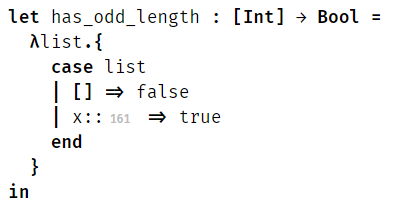
\includegraphics[scale=0.45,valign=t]{imgs/maybe_exhaustive.png}%
    \vphantom{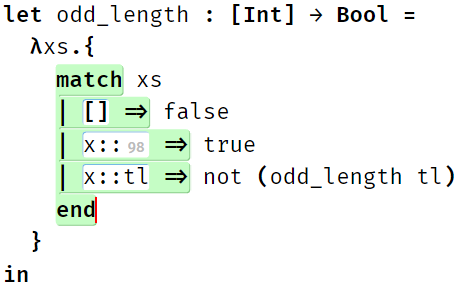
\includegraphics[scale=0.45,valign=t]{imgs/maybe_inexhaustive.png}}
}
\hfil
  \subfloat[Necessarily Inexhaustive\label{fig:not-exhautive}]{
    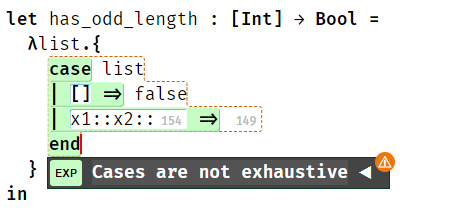
\includegraphics[scale=0.45,valign=t]{imgs/not_exhaustive.png}
    \vphantom{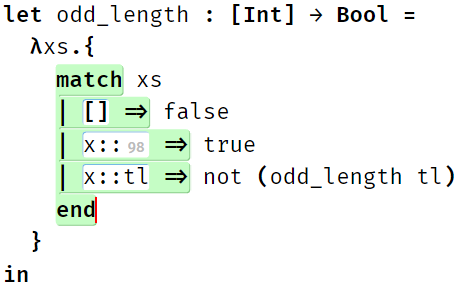
\includegraphics[scale=0.45,valign=t]{imgs/maybe_inexhaustive.png}}
}
\hfil
  \subfloat[Necessarily Exhaustive\label{fig:yes-inexhautive}]{
    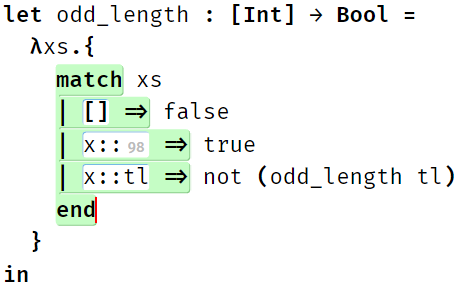
\includegraphics[scale=0.45,valign=t]{imgs/maybe_inexhaustive.png}
}
  \caption{Exhaustiveness Checking with Pattern Holes}
  \label{fig:exhaustiveness}
\end{figure}

We begin with the editor state in Fig.~\ref{fig:may-exhaustive}, 
where there is a hole in the tail position of the cons (\li{::}) pattern.
In determining whether this \li{match} expression is exhaustive, we 
must reason over all potential hole fillings. In this case, the 
\li{match} expression is \emph{indeterminately exhaustive}, because there are hole fillings,
such as a pattern variable \li{tl}, that would result in a determination
of exhaustiveness, while there are other hole fillings, such as \li{[]} or \li{y::tl},
where the determination would instead be inexhaustiveness. In the Hazel user interface, we choose to alert the programmer with an error
indicator only when the \li{match} expression is necessarily inexhaustive,
so no error appears for this editor state. The motivation for this choice is that we do not want to draw the programmer's attention for a problem that may or may not actually persist once the user has filled the holes. The cursor inspector does, however, provide typing information for the pattern hole when the programmer places their cursor there, as seen in Fig.~\ref{fig:may-exhaustive}. This and other pattern holes can be typed using information about how they are used. In this example, Hazel can determine that the pattern hole must have type \li{[Int]} because that is the only valid type for the right-hand side of the cons pattern when we are matching on \li{xs}, which is of type \li{[Int]}.

While pattern holes can make it impossible to conclusively determine the exhaustiveness of a \li{match} expression, the mere presence of a pattern hole does not mean that exhaustiveness errors never arise. Consider now
the editor state in Fig.~\ref{fig:not-exhautive}. In this case,
although there are again pattern holes in the second pattern, 
it can be determined that this \li{match} expression is \emph{necessarily inexhaustive}
because no matter how those holes are filled, this \li{match} expression will fail to 
match lists with exactly one element (singleton lists). Since this \li{match} expression is inexhaustive no matter how the holes are filled,
we alert the user with an error indicator and an error message when the cursor is on the \li{match} expression.


It is also possible for a \li{match} expression with pattern holes to be \emph{necessarily exhaustive}, as seen in Fig.~\ref{fig:yes-inexhautive}. Here, the first and third pattern are
exhaustive, regardless of how the hole in the second pattern is filled (e.g. with \li{[]} to special case singleton lists). We choose not to visually distinguish between necessarily and indeterminately exhaustive \li{match} expressions, again to avoid drawing
the programmer's attention to information that is unlikely to be actionable, but the
underlying semantic distinction is interesting to observe.

\subsection{Redundancy Checking with Pattern Holes}
\label{sec:hazel-redundancy}
A pattern is redundant if, for every value of the scrutinee's type that match that pattern, one of the preceding patterns in the \li{match} expression will necessarily 
match it. In the presence of pattern holes, we again have to consider all possible hole fillings in this analysis, leading to three possibilities: \emph{necessarily irredundant}, \emph{indeterminately irredundant}, and \emph{necessarily redundant} patterns.

In the editor state in Fig.~\ref{fig:may-redundant}, there is a pattern hole in the \emph{second} pattern of the \li{match} expression. It is possible to fill this hole in a way that would make the \emph{third} pattern irredundant, such as the empty list pattern, \texttt{[]}. 
However, it is also possible that the hole could be filled in a way that causes the third pattern to become redundant, such as the cons pattern \texttt{y::tl}. Consequently, the third pattern in this \li{match} expression is indeterminately irredundant (we chose ``irredundant'' rather than ``redundant'' in this phrase because, like exhaustiveness, irredundancy is the programmer's goal).

The second pattern itself, although it contains a pattern hole, is necessarily irredundant because no matter how the hole is filled, the first pattern, \li{[]}, does not overlap with it. The first pattern is always necessarily irredundant, even when it is a hole, because
there are no previous patterns (except if the scrutinee has the nullary sum, i.e. \li{void}, type, which has no values; see Supplementary Material).

The editor state in Fig.~\ref{fig:must-redundant} shows that a pattern with a hole can nevertheless be determined to be necessarily redundant.
In this case, the previous pattern handles every non-empty list, so no matter how the pattern hole is filled, it will be redundant.
Indeed, even an empty hole pattern in the third pattern would be redundant because the two preceding patterns are exhaustive.
 As with exhaustiveness, we only alert
the user to necessarily redundant patterns, so this is the only pattern in Fig.~\ref{fig:redundancy} where an error is reported.

\begin{figure}
    \begin{subfigure}[t]{0.45\textwidth}
    \centering
    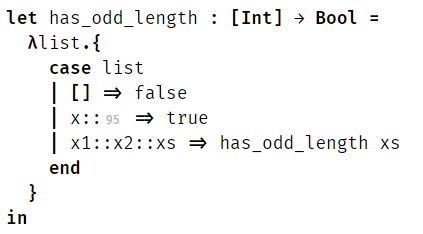
\includegraphics[scale=0.5,valign=t]{imgs/maybe_redundant.png}%
    \vphantom{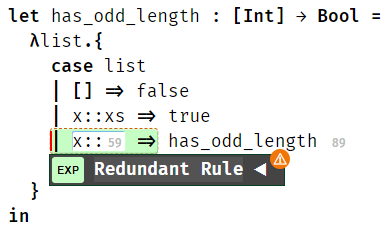
\includegraphics[scale=0.5,valign=t]{imgs/redundant.png}}
    \vspace{-6px}
    \caption{Necessarily Irredundant (first two patterns) + Indeterminately Irredundant (third pattern)\label{fig:may-redundant}}
    \end{subfigure}
    \begin{subfigure}[t]{0.45\textwidth}
    \centering
  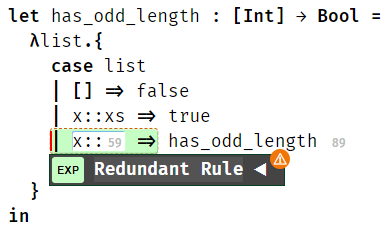
\includegraphics[scale=0.5,valign=t]{imgs/redundant.png}
  \vspace{-6px}
  \caption{Necessarily Redundant (third pattern) \label{fig:must-redundant}}
  \end{subfigure}
  \vspace{-3px}
  \caption{Redundancy Checking with Pattern Holes}
  \vspace{-3px}
  \label{fig:redundancy}
\end{figure}


\subsection{Live Evaluation with Expression and Pattern Holes}
\label{sec:hazel-live-eval}
In the examples above, we considered only {static analysis} of programs with pattern holes.
However, Hazel also supports live evaluation with holes, proceeding ``around'' holes
as necessary to produce a result with a possibly \emph{indeterminate value}, i.e. an expression that might retain holes in critical elimination positions \cite{DBLP:journals/pacmpl/OmarVCH19}.%\cite{DBLP:journals/tocl/NanevskiPP08}.

In a language without holes, the value of the scrutinee can be determined to either \emph{match} or \emph{mismatch} every pattern of the same type.
In order to support live evaluation with both expression and pattern holes, we have to consider now a third possiblilty: an \emph{indeterminate match} between the scrutinee, which may itself have an indeterminate value, and a pattern. Let us consider the possibilities in Fig.~\ref{fig:evaluation-ex}. 

We first look in Fig.~\ref{fig:exp-hole} at the situation where there are expression holes but no pattern holes. 
We see in \autoref{fig:exp-hole} that the argument to \li{odd_length} has a hole, so evaluation cannot determine a unique value. Instead,
the argument has an \emph{indeterminate value}. 
When we proceed through pattern matching, we can only make decisions that would be valid no matter how the hole in the tail of the list
would be filled. 
We can determine that the first pattern, \li{[]}, necessarily mismatches since the argument is not empty. 
Similarly, we can also determine that the second pattern necessarily mismatches because regardless of how the hole is filled, the list is at least of length two. 
When checking the third pattern, we see that this matches any list of at least two elements.
We know that the scrutinee necessarily matches this pattern, binding \li{tl} to whatever the hole is filled with, so we can take this branch. We next proceed to recurse, now with the hole itself as the argument. In the recursive call, we cannot determine whether the first pattern, \li{[]}, matches, since the empty expression hole could be filled with \li{[]} or with any other list. This indeterminate match leaves the entire \li{match} expression with an indeterminate value, and we cannot proceed any further as shown in the
evaluation result at the bottom of Fig.~\ref{fig:exp-hole}.

\begin{figure}
\begin{subfigure}[t]{0.45\textwidth}
\centering
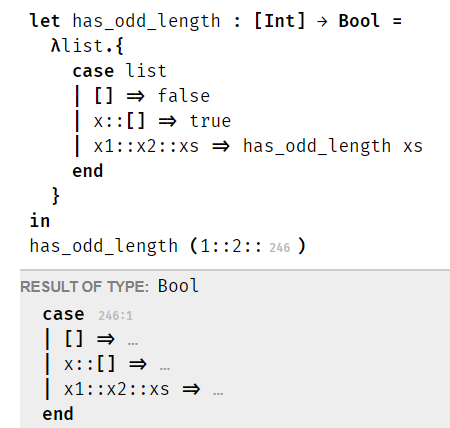
\includegraphics[scale=0.47,valign=t]{imgs/pat_match_exp_holes.png}\vphantom{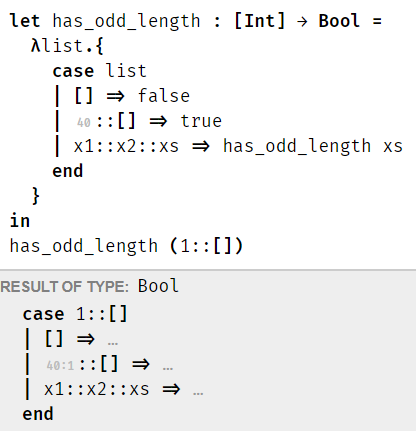
\includegraphics[scale=0.47,valign=t]{imgs/pat_match_pat_holes.png}}
\caption{Pattern matching with expression holes\label{fig:exp-hole}}
\end{subfigure}
\begin{subfigure}[t]{0.45\textwidth}
\centering
{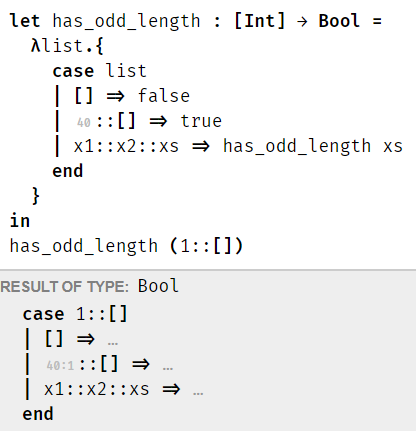
\includegraphics[scale=0.47,valign=t]{imgs/pat_match_pat_holes.png}}
\caption{Pattern matching with pattern holes\label{fig:pat-hole}}
\end{subfigure}
\vspace{-3px}
  \caption{Live Evaluation with Expression and Pattern Holes}
  \vspace{-3px}
  \label{fig:evaluation-ex}
\end{figure}


Next we consider in \autoref{fig:pat-hole} the situation where there are (several) pattern holes encountered during evaluation. 
We know that the first pattern, \li{[]}, necessarily mismatches the scrutinee, \li{1::[]}, for the standard reasons.
The second pattern, which contains two holes but which matches only lists of length two, also necessarily mismatches the scrutinee.
The third pattern matches singleton lists, like the scrutinee. However, a pattern hole appears at the pattern's head, so it cannot be determined 
whether there is necessarily a match or a mismatch with \li{1::[]}. For example, if the pattern hole is filled with the pattern \li{2}, 
then there would be a mismatch. Alternatively, if the pattern hole is filled with the pattern \li{x}, then there would be a match. This indeterminate match causes the \li{match} expression itself to have an indeterminate value.
However, by graying out mismatched rules in the result, we can report to the programmer how far match evaluation was able to proceed, as shown at the bottom of Fig.~\ref{fig:pat-hole}.
\section{Peanut: The Core Calculus}
% We now formalize the intuitions developed in \autoref{sec:examples} as a core calculus that supports pattern matching with typed holes in both expression and pattern position.
Traditional matching of an expression to a pattern leads to success or failure (or divergence in the lazy setting). In the setting of typed holes, there is an additional outcome: \emph{indeterminate}.
An indeterminate match occurs when the pattern or expression contains holes and the match would succeed or fail depending on how the programmer modifies those holes. Such dependence on yet unspecified programmer input similarly colors the outcomes of corresponding coverage and redundancy checkers: a collection of patterns may be \emph{indeterminately inexhaustive}, and a pattern may be \emph{indeterminately redundant} with respect to some preceding collection of patterns.

In this section, we formalize these concepts in a core calculus called Peanut that supports pattern matching with typed holes in both expression and pattern position. 
We begin with the syntax of the calculus in \autoref{sec:Syntax}\todo{change autoref settings to say Sec. 3.1 instead of subsection 3.1}.
In \autoref{sec:dynamics}, we define the dynamic semantics as a small-step operational semantics with support for evaluating incomplete programs.
Next, in \autoref{sec:statics}, we define a corresponding static semantics as a type assignment system together with a match constraint language that we use to reason hypothetically about exhaustiveness and redundancy in the presence of
holes.
Finally, in \autoref{sec:algorithm}, we give an algorithmic formulation of the exhaustiveness and redundancy checker and prove it sound with respect to the declarative formulation.

% !TEX root= pattern-paper.tex

\begin{figure}[ht]
    \centering
    \begin{minipage}{.5\linewidth}
  $\arraycolsep=4pt\begin{array}{lll}
    e & ::= &
      x ~\vert~
      \hnum{n} \\
      & ~\vert~ &
      \hlam{x}{\tau}{e} ~\vert~
      \hap{e_1}{e_2} \\
      & ~\vert~ &
      \hpair{e_1}{e_2} ~\vert~
      \hfst{e} ~\vert~ \hsnd{e} \\
      & ~\vert~ &
      \hinl{\tau}{e} ~\vert~
      \hinr{\tau}{e} \\
      & ~\vert~ &
      \hmatch{e}{\hat{rs}} \\
      & ~\vert~ &
      \hehole{u} ~\vert~
      \hhole{e}{u} \\
    \end{array}$
    \end{minipage}%
    \begin{minipage}{.5\linewidth}
  $\arraycolsep=4pt\begin{array}{lll}
    \tau & ::= &
      \tnum ~\vert~
      \tarr{\tau_1}{\tau_2} ~\vert~
      \tprod{\tau_1}{\tau_2} ~\vert~
      \tsum{\tau_1}{\tau_2} \\
    \hat{rs} & ::= &
      \zrulsP{rs}{r}{rs} \\
    rs & ::= &
      \cdot ~\vert~ \hrulesP{r}{rs'} \\
    r & ::= &
      \hrul{p}{e} \\
    p & ::= &
      x ~\vert~
      \_ ~\vert~
      \hnum{n} ~\vert~
      \hpair{p_1}{p_2} \\
      & ~\vert~ &
      \hinlp{p} ~\vert~
      \hinrp{p} ~\vert~
      \heholep{w} ~\vert~
      \hholep{p}{w}{\tau}
    \end{array}$
    \end{minipage}
\caption{Syntax}
\label{fig:syntax}
\end{figure}
% !TEX root= pattern-paper.tex

\begin{figure}[ht]

\judgbox{\rmpointer{\zrules} = rs}
        {$rs$ can be obtained by erasing pointer from $\zrules$}
\begin{align*}
  \rmpointer{\zruls{\cdot}{r}{rs}} &= \hrules{r}{rs} \\
  \rmpointer{\zruls{\hrulesP{r'}{rs'}}{r}{rs}} &= \hrules{r'}{\rmpointer{\zruls{rs'}{r}{rs}}}
\end{align*}

\caption{Pointer Eraser flattens the rules with pointer.}
\label{fig:pointer-eraser}
\end{figure}


\subsection{Syntax}
\label{sec:Syntax}
\figurename~\ref{fig:syntax} presents the syntax of Peanut.
Peanut is based on the internal language of Hazelnut Live, a typed lambda calculus featuring holes in expression position \cite{DBLP:journals/pacmpl/OmarVCH19}.
We choose numbers as the base type and add binary sums and binary products so that we have interesting
patterns to consider. We also remove the machinery related to gradual typing (casts and failed casts) to focus our attention on pattern matching in particular. Most forms are standard (we base our formulation on \cite{Harper2012}). We include functions, function application, pairs, explicit projection operators (for reasons we will consider below), and left and right injections, which are the introductory forms for sum types. Functions and injections include type annotations so that we can define a simple type assignment system. The forms of particular interest here are holes and match expressions.

Empty expression holes are written $\hehole{u}$ and non-empty expression holes, which serve as membranes around type inconsistencies, are written $\hhole{e}{u}$. Similarly, empty pattern holes are written $\hehole{w}$ and non-empty pattern holes, which are analogous, are written $\hhole{p}{w}$. Here, $u$ are expression hole identifiers and $w$ are pattern hole identifiers.
We are modeling an internal language, so we assume that hole identifiers 
correspond to unique holes in the user's original program, which we do not model here. We do not impose a uniqueness constraint, however, because a hole can 
appear multiple times during evaluation due to substitution.

A match expression, $\hmatch{e}{\zrules}$, 
consists of a scrutinee, $e$, and a zipper of rules, $\zrules$, i.e. a sequence of one or more rules with a pointer marking the rule currently being considered during evaluation (we assume that the marker is on the first rule initially). Syntactically, this is a triple, $\zruls{rs_{pre}}{r}{rs_{post}}$, consisting of a prefix rule sequence, $rs_{pre}$, a current rule, $r$, and a suffix rule sequence, $rs_{post}$. We can erase the pointer using the pointer erasure operator, $\rmpointer{\zrules}$, defined in \autoref{fig:pointer-eraser}. 
Each rule, $r$, consists of a pattern and an expression, which we call the branch expression.



\subsection{Dynamic Semantics}\label{sec:dynamics}

% !TEX root= pattern-paper.tex

\begin{figure}[ht]

\judgbox{\htrans{e}{e'}}{$e$ takes a step to $e'$}

\begin{mathpar}
\Infer{\ITHole}{
  \htrans{e}{e'}
}{
  \htrans{\hhole{e}{u}}{\hhole{e'}{u}}
}

\Infer{\ITApFun}{
  \htrans{e_1}{e_1'}
}{
  \htrans{\hap{e_1}{e_2}}{\hap{e_1'}{e_2}}
}

\Infer{\ITApArg}{
  \isFinal{e_1} \\
  \htrans{e_2}{e_2'}
}{
  \htrans{\hap{e_1}{e_2}}{\hap{e_1}{e_2'}}
}

\Infer{\ITAp}{
  \isFinal{e_2}
}{
  \hap{\hlam{x}{\tau}{e_1}}{e_2} \mapsto
    [e_2/x]e_1
}

\Infer{\ITPairL}{
  \htrans{e_1}{e_1'}
}{
  \htrans{\hpair{e_1}{e_2}}{\hpair{e_1'}{e_2}}
}

\Infer{\ITPairR}{
  \isFinal{e_1} \\
  \htrans{e_2}{e_2'}
}{
  \htrans{\hpair{e_1}{e_2}}{\hpair{e_1}{e_2'}}
}

\Infer{\ITPrl}{
  \isFinal{\hpair{e_1}{e_2}}
}{
  \htrans{\hprl{\hpair{e_1}{e_2}}}{e_1}
}

\Infer{\ITPrr}{
  \isFinal{\hpair{e_1}{e_2}}
}{
  \htrans{\hprr{\hpair{e_1}{e_2}}}{e_2}
}

\Infer{\ITInl}{
  \htrans{e}{e'}
}{
  \htrans{\hinl{\tau}{e}}{\hinl{\tau}{e'}}
}

\Infer{\ITInr}{
  \htrans{e}{e'}
}{
  \htrans{\hinr{\tau}{e}}{\hinr{\tau}{e'}}
}

\Infer{\ITExpMatch}{
  \htrans{e}{e'}
}{
  \htrans{\hmatch{e}{\zrules}}{\hmatch{e'}{\zrules}}
}

\Infer{\ITSuccMatch}{
  \isFinal{e} \\
  \hpatmatch{e}{p_r}{\theta}
}{
  \htrans{
    \hmatch{e}{\zruls{rs_{pre}}{\hrulP{p_r}{e_r}}{rs_{post}}}
  }{
    [\theta](e_r)
  }
}

\Infer{\ITFailMatch}{
  \isFinal{e} \\
  \hnotmatch{e}{p_r}
}{
  \htrans{
    \hmatch{e}{\zruls{rs}{\hrulP{p_r}{e_r}}{\hrulesP{r'}{rs'}}}
  }{
    \hmatch{e}{
      \zruls{
        \rmpointer{\zruls{rs}{\hrulP{p_r}{e_r}}{\cdot}}
      }{r'}{rs'}
    }
  }
}
\end{mathpar}

  \caption{Stepping}
  \label{fig:step}
\end{figure}

% !TEX root= pattern-paper.tex

\begin{figure}[th]

\judgbox{\isVal{e}}{$e$ is a value}

\begin{mathpar}
\Infer{\VNum}{ }{
  \isVal{\hnum{n}}
}

\Infer{\VLam}{ }{
  \isVal{\hlam{x}{\tau}{e}}
}

\Infer{\VPair}{
  \isVal{e_1} \\
  \isVal{e_2}
}{
  \isVal{\hpair{e_1}{e_2}}
}

\Infer{\VInl}{
  \isVal{e}
}{
  \isVal{\hinl{\tau}{e}}
}

\Infer{\VInr}{
  \isVal{e}
}{
  \isVal{\hinr{\tau}{e}}
}
\end{mathpar}

\judgbox{\isIndet{e}}{$e$ is indeterminate}

\begin{mathpar}
\Infer{\IEHole}{ }{
  \isIndet{\hehole{u}}
}

\Infer{\IHole}{
  \isFinal{e}
}{
  \isIndet{\hhole{e}{u}}
}

\Infer{\IAp}{
  \isIndet{e_1} \\ \isFinal{e_2}
}{
  \isIndet{\hap{e_1}{e_2}}
}

\Infer{\IPairL}{
  \isIndet{e_1} \\ \isVal{e_2}
}{
  \isIndet{\hpair{e_1}{e_2}}
}

\Infer{\IPairR}{
  \isVal{e_1} \\ \isIndet{e_2}
}{
  \isIndet{\hpair{e_1}{e_2}}
}

\Infer{\IPair}{
  \isIndet{e_1} \\ \isIndet{e_2}
}{
  \isIndet{\hpair{e_1}{e_2}}
}

\Infer{\IFst}{
  \isIndet{e} \\ e \neq \hpair{e_1}{e_2}
}{
  \isIndet{\hfst{e}}
}

\Infer{\ISnd}{
  \isIndet{e} \\ e \neq \hpair{e_1}{e_2}
}{
  \isIndet{\hsnd{e}}
}

\Infer{\IInl}{
  \isIndet{e}
}{
  \isIndet{\hinl{\tau}{e}}
}

\Infer{\IInr}{
  \isIndet{e}
}{
  \isIndet{\hinr{\tau}{e}}
}

\Infer{\IMatch}{
  \isFinal{e} \\
  \hmaymatch{e}{p_r}
}{
  \isIndet{
    \hmatch{e}{\zruls{rs_{pre}}{\hrulP{p_r}{e_r}}{rs_{post}}}
  }
}
\end{mathpar}

\judgbox{\isFinal{e}}{$e$ is final}

\begin{mathpar}
\Infer{\FVal}{
  \isVal{e}
}{
  \isFinal{e}
}

\Infer{\FIndet}{
  \isIndet{e}
}{
  \isFinal{e}
}
\end{mathpar}

  \caption{Final expressions}
  \label{fig:final}
\end{figure}


Hazelnut Live \cite{DBLP:journals/pacmpl/OmarVCH19} features a dynamic semantics capable of evaluating expressions with holes.
Rather than stopping upon encountering a hole, evaluation proceeds around it, taking all evaluation steps that do not depend on the eventual contents of the hole.
\autoref{fig:step} presents the corresponding stepping judgment $\htrans{e}{e'}$ of Peanut, many of the rules of which are directly adapted from Hazelnut Live.\footnote{Hazelnut Live is a contextual small-step semantics, whereas we choose to define a standard small-step semantics for Peanut.}
The rules of interest in this work are those concerning match expressions, namely (match rules\todo{}).
These inference rules use the zipper representation of the Peanut syntax to record the pattern matching progress.

We use zipper rules of the form $\zrulsP{rs}{r}{rs}$ in match expressions to represent the intermediate states when we are performing pattern matching.
The former $rs$ represents the preceding rules that has already been considered and fails to match the scrutinee; the rule $r$ in the middle represents the current rule being considered; the latter $rs$ represents the remaining rules to be considered.
\figurename~\ref{fig:pointer-eraser} defines a helper function to flatten the zipper rules.
If we need to move the rule pointer to the next rule, we can append the current rule after the preceding rules, and regard the initial rule in the remaining rule as the new current rule.
The conclusion of Rule \ITFailMatch demonstrates how it works.
\todo{edit this paragraph, bringing up successful and failed matches in connection to traditional pattern matching. possibly note some details regarding finality of match scrutinee. see commented text.}
% \figurename~\ref{fig:step} defines the stepping judgment
% $\htrans{e}{e'}$. We will focus on stepping judgments of match expressions.
% Rule \ITExpMatch specifies that the match expression can take a step as its its
% scrutinee can take a step. Note that Rule \ITFailMatch and Rule \ITSuccMatch
% share the premise, $\isFinal{e}$, which is defined in \figurename~\ref{fig:final}. It
% means that expression $e$ is \textit{final} in the sense that it is either already a
% \textit{value} or \textit{indeterminate}, \ie, cannot be evaluated further due to unfilled holes
% \cite{DBLP:journals/pacmpl/OmarVCH19}. And only when the scrutinee is final,
% shall we consider the constinuent rules of the match expression in order. As in
% the examples shown in \listfigurename~\ref{fig:exp-hole-step},\ref{fig:pat-hole-step},

% \begin{itemize}
%   \item
%     if the final scrutinee does not match the pattern in the current rule,
%     then we move the pointer to the next rule (Rule \ITFailMatch)

%   \item
%     if the final scrutinee does match the pattern in the current rule, 
%     then we take the emitted substitution $\theta$ and apply it on the subexpression of that rule (Rule \ITSuccMatch)

%   \item 
%     if the final scrutinee may or may not match the pattern in the current rule,
%     then the match expression is said to be indeterminate (Rule \IMatch)
% \end{itemize}


The final result $e$ of evaluation may be, as characterized by the judgment $\isFinal{e}$ in \autoref{fig:final}, either a value ($\isVal{e}$) or an \emph{indeterminate} form ($\isIndet{e}$) whose continued evaluation depends on the remaining holes' contents. For example, Rules \IAp and \IEHole together derive that a function application with a hole in function position is indeterminate.

% !TEX root= pattern-paper.tex

\begin{figure}[!b]

\judgbox{
  \hpatmatch{e}{p}{\theta}
}{
  $e$ matches $p$, emitting $\theta$
}

\begin{mathpar}
\Infer{\MVar}{ }{
  \hpatmatch{e}{x}{e / x}
}

\Infer{\MWild}{ }{
  \hpatmatch{e}{\_}{\cdot}
}

\Infer{\MNum}{ }{
  \hpatmatch{\hnum{n}}{\hnum{n}}{\cdot}
}

\Infer{\MPair}{
  \hpatmatch{e_1}{p_1}{\theta_1} \\
  \hpatmatch{e_2}{p_2}{\theta_2}
}{
  \hpatmatch{\hpair{e_1}{e_2}}{\hpair{p_1}{p_2}}{\theta_1 \uplus \theta_2}
}

\Infer{\MInl}{
  \hpatmatch{e}{p}{\theta}
}{
  \hpatmatch{\hinl{\tau}{e}}{\hinlp{p}}{\theta}
}

\Infer{\MInr}{
  \hpatmatch{e}{p}{\theta}
}{
  \hpatmatch{\hinr{\tau}{e}}{\hinrp{p}}{\theta}
}

\Infer{\MNotIntroPair}{
  \notIntro{e} \\
  \hpatmatch{\hprl{e}}{p_1}{\theta_1} \\
  \hpatmatch{\hprr{e}}{p_2}{\theta_2}
}{
  \hpatmatch{e}{\hpair{p_1}{p_2}}{\theta_1 \uplus \theta_2}
}
\end{mathpar}

\judgbox{
  \hnotmatch{e}{p}
}{
  $e$ does not match $p$
}

\begin{mathpar}

\Infer{\NMNum}{
  n_1 \neq n_2
}{
  \hnotmatch{\hnum{n_1}}{\hnum{n_2}}
}

\Infer{\NMPairL}{
  \hnotmatch{e_1}{p_1}
}{
  \hnotmatch{\hpair{e_1}{e_2}}{\hpair{p_1}{p_2}}
}

\Infer{\NMPairR}{
  \hnotmatch{e_2}{p_2}
}{
  \hnotmatch{\hpair{e_1}{e_2}}{\hpair{p_1}{p_2}}
}

\Infer{\NMConfL}{ }{
  \hnotmatch{\hinr{\tau}{e}}{\hinlp{p}}
}

\Infer{\NMConfR}{ }{
  \hnotmatch{\hinl{\tau}{e}}{\hinrp{p}}
}

\Infer{\NMInl}{
  \hnotmatch{e}{p}
}{
  \hnotmatch{\hinr{\tau}{e}}{\hinlp{p}}
}

\Infer{\NMInr}{
  \hnotmatch{e}{p}
}{
  \hnotmatch{\hinl{\tau}{e}}{\hinrp{p}}
}
\end{mathpar}

\judgbox{
  \hmaymatch{e}{p}
}{
  $e$ indeterminately matches $p$
}

\begin{mathpar}
\Infer{\MMEHole}{ }{
  \hmaymatch{e}{\heholep{w}}
}

\Infer{\MMHole}{ }{
  \hmaymatch{e}{\hholep{p}{w}{\tau}}
}
\\
\Infer{\MMNotIntro}{
  \notIntro{e} \\
  \refutable{p}
}{
  \hmaymatch{e}{p}
}

\Infer{\MMPairL}{
  \hmaymatch{e_1}{p_1} \\
  \hpatmatch{e_2}{p_2}{\theta_2}
}{
  \hmaymatch{\hpair{e_1}{e_2}}{\hpair{p_1}{p_2}}
}

\Infer{\MMPairR}{
  \hpatmatch{e_1}{p_1}{\theta_1} \\
  \hmaymatch{e_2}{p_2}
}{
  \hmaymatch{\hpair{e_1}{e_2}}{\hpair{p_1}{p_2}}
}

\Infer{\MMPair}{
  \hmaymatch{e_1}{p_1} \\
  \hmaymatch{e_2}{p_2}
}{
  \hmaymatch{\hpair{e_1}{e_2}}{\hpair{p_1}{p_2}}
}

\Infer{\MMInl}{
  \hmaymatch{e}{p}
}{
  \hmaymatch{\hinl{\tau}{e}}{\hinlp{p}}
}

\Infer{\MMInr}{
  \hmaymatch{e}{p}
}{
  \hmaymatch{\hinr{\tau}{e}}{\hinrp{p}}
}
\end{mathpar}

\caption{Three possible outcomes of pattern matching}
\label{fig:patmatch}
\end{figure}


Peanut extends this concept of indeterminacy to pattern matching.
\autoref{fig:patmatch} presents the three possible outcomes of matching an expression $e$ to a pattern $p$.
First, the judgment $\hpatmatch{e}{p}{\theta}$ denotes a successful match as witnessed by the substitution $\theta$ consisting of the variables bound in $p$. Second, the judgment $\hnotmatch{e}{p}$ denotes that $e$ does not match $p$. Third, the judgment $\hmaymatch{e}{p}$ indicates an \emph{indeterminate match} due to the presence of holes in $e$ or $p$.
\todo{add mention of assupmtion of finality of expression}
\todo{recall how we saw how successful/failed matches contextualize within stepping judgment, note how indeterminate match appears in indet judgment}
% \figurename~\ref{fig:patmatch} defines three judgments corresponding to the
% three possible results of pattern matching. We consider a final scrutinee $e$
% and a pattern $p$ that are of the same type (see \autoref{sec:statics}). \autoref{fig:notintro} defines the judgment for expressions that cannot be values by simply looking at its form. Hence, when some final expression is of such form, they must be indeterminate. Besides, there is not need to recursively consider its inner expression during pattern matching.


\todo{add paragraph opener here bridging to going into some detail regarding specifics of matching}

% !TEX root= pattern-paper.tex

\begin{figure}[!ht]
\judgbox{
  \refutable{p}
}{$p$ is refutable}

\begin{mathpar}
\Infer{\RNum}{ }{
  \refutable{\hnum{n}}
}

\Infer{\REHole}{ }{
  \refutable{\heholep{w}}
}

\Infer{\RHole}{ }{
  \refutable{\hholep{p}{w}{\tau}}
}

\Infer{\RInl}{ }{
  \refutable{\hinlp{p}}
}

\Infer{\RInr}{ }{
  \refutable{\hinrp{p}}
}

\Infer{\RPairL}{
  \refutable{p_1}
}{
  \refutable{\hpair{p_1}{p_2}}
}

\Infer{\RPairR}{
  \refutable{p_2}
}{
  \refutable{\hpair{p_1}{p_2}}
}
\end{mathpar}
\caption{Refutable Patterns}
\label{fig:refutable}
\end{figure}
% !TEX root= pattern-paper.tex

\begin{figure}[ht]
\judgbox{
  \notIntro{e}
}{
  $e$ cannot be a value syntactically
}

\begin{mathpar}
\Infer{NVEHole}{ }{
  \notIntro{\hehole{u}}
}

\Infer{NVHole}{ }{
  \notIntro{\hhole{e}{u}}
}

\Infer{NVAp}{ }{
  \notIntro{\hap{e_1}{e_2}}
}

\Infer{NVMatch}{ }{
  \notIntro{\hmatch{e}{\zrules}}
}

\Infer{NVPrl}{ }{
  \notIntro{\hprl{e}}
}

\Infer{NVPrr}{ }{
  \notIntro{\hprr{e}}
}
\end{mathpar}

  \caption{Expressions that are syntactically not values}
  \label{fig:notintro}
\end{figure}

\todo{this paragraph below is floating content, needs to be worked into its surroundings}
The judgment $\hpatmatch{e}{p}{\theta}$ denotes that $e$ matches $p$, as witnessed by
the substitution $\theta$ defined on the variables in $p$, while the judgment
$\hnotmatch{e}{p}$ denotes that $e$ does not match $p$. Notably, we introduce the
third possibility $\hmaymatch{e}{p}$ --- $e$ may match $p$, which is also the
\textit{key concept}
\todo{d: the concept itself should be emphasized (if at all), not the phrase ``key concept''}
in pattern matching with holes. Rules \MMEHole and \MMHole
specify that any final expression may match a pattern hole, regardless of
whether it is empty or non-empty. On the other hand, Rule \MMNotIntro specifies that
an indeterminate expression may match a pattern $p$ only when $p$ is refutable
(see \figurename~\ref{fig:refutable}).
It is because any final expressions
must match an irrefutable pattern of the same type, and it does not make sense to allow
$\hpatmatch{e}{p}{\theta}$ and $\hmaymatch{e}{p}$ to be derivable at the same time.
Actually,
the three possible results of pattern matching are mutually exclusive and at
least one of judgments can be derived under certain assumptions, as shown in the
following lemma.

The judgment $\hexptyp{\Gamma}{\Delta}{e}{\tau}$ specifies that expression $e$ is well-typed. And the judgment $\hpattyp{p}{\tau}{\Gamma}{\Delta}$ specifies that we can assign type $\tau$ to pattern $p$.
\begin{lemma}[Matching Determinism]
  \label{lemma:match-determinism}
  If $\isFinal{e}$ and $\hexptyp{\cdot}{\Delta}{e}{\tau}$ and $\hpattyp{p}{\tau}{\Gamma}{\Delta}$ then exactly one of the following holds
  \begin{enumerate}
    \item $\hpatmatch{e}{p}{\theta}$ for some $\theta$
    \item $\hmaymatch{e}{p}$
    \item $\hnotmatch{e}{p}$
  \end{enumerate}
\end{lemma}

The determinism of pattern matching ensures the determinism of dynamic semantics.

\begin{theorem}[Determinism]
  \label{theorem:determinism}
  If $\hexptyp{\cdot}{\Delta}{e}{\tau}$ then exactly one of the following holds
  \begin{enumerate}
    \item $\isVal{e}$
    \item $\isIndet{e}$
    \item $\htrans{e}{e'}$ for some unique $e'$
  \end{enumerate}
\end{theorem}
\todo{prove unique e'?}

\subsection{Static Semantics}\label{sec:statics}

% !TEX root= pattern-paper.tex

\begin{figure}[ht]
\judgbox{
  \hexptyp{\Gamma}{\Delta}{e}{\tau}
}{
  $e$ is of type \(\tau\)
}
  \begin{mathpar}
%  \Infer{\TVar}{ }{
%    \hexptyp{\Gamma, x:\tau}{\Delta}{x}{\tau}
%  }
%
%  \Infer{\TEHole}{ }{
%    \hexptyp{\Gamma}{\Delta, u::\tau}{\hehole{u}}{\tau}
%  }
%
%  \Infer{\THole}{
%    \hexptyp{\Gamma}{\Delta, u::\tau}{e}{\tau'}
%  }{
%    \hexptyp{\Gamma}{\Delta, u::\tau}{\hhole{e}{u}}{\tau}
%  }
%
%  \Infer{\TNum}{ }{
%    \hexptyp{\Gamma}{\Delta}{\hnum{n}}{\tnum}
%  }
%
%  \Infer{\TLam}{
%    \hexptyp{\Gamma, x:\tau_1}{\Delta}{e}{\tau_2}
%  }{
%    \hexptyp{\Gamma}{\Delta}{\hlam{x}{\tau_1}{e}}{\tarr{\tau_1}{\tau_2}}
%  }
%
%  \Infer{\TAp}{
%    \hexptyp{\Gamma}{\Delta}{e_1}{\tarr{\tau_2}{\tau}} \\
%    \hexptyp{\Gamma}{\Delta}{e_2}{\tau_2}
%  }{
%    \hexptyp{\Gamma}{\Delta}{\hap{e_1}{e_2}}{\tau}
%  }
%
%  \Infer{\TPair}{
%    \hexptyp{\Gamma}{\Delta}{e_1}{\tau_1} \\
%    \hexptyp{\Gamma}{\Delta}{e_2}{\tau_2}
%  }{
%    \hexptyp{\Gamma}{\Delta}{\hpair{e_1}{e_2}}{\tprod{\tau_1}{\tau_2}}
%  }
%
%  \Infer{\TFst}{
%    \hexptyp{\Gamma}{\Delta}{e}{\tprod{\tau_1}{\tau_2}}
%  }{
%    \hexptyp{\Gamma}{\Delta}{\hfst{e}}{\tau_1}
%  }
%  
%  \Infer{\TSnd}{
%    \hexptyp{\Gamma}{\Delta}{e}{\tprod{\tau_1}{\tau_2}}
%  }{
%    \hexptyp{\Gamma}{\Delta}{\hsnd{e}}{\tau_2}
%  }
%  
%  \Infer{\TInl}{
%    \hexptyp{\Gamma}{\Delta}{e}{\tau_1}
%  }{
%    \hexptyp{\Gamma}{\Delta}{\hinl{\tau_2}{e}}{\tsum{\tau_1}{\tau_2}}
%  }
%
%  \Infer{\TInr}{
%    \hexptyp{\Gamma}{\Delta}{e}{\tau_2}
%  }{
%    \hexptyp{\Gamma}{\Delta}{\hinr{\tau_1}{e}}{\tsum{\tau_1}{\tau_2}}
%  }
  
  \Infer{TMatchZPre}{
    \hexptyp{\Gamma}{\Delta}{e}{\tau} \\
    \chrulstyp{\Gamma}{\Delta}{\cfalsity}{\hrules{r}{rs}}{\tau}{\xi}{\tau'} \\
    \csatisfyormay{\ctruth}{\xi}
  }{
  \hexptyp{\Gamma}{\Delta}{\hmatch{e}{\zruls{\cdot}{r}{rs}}}{\tau'}
  }

  \Infer{TMatchNZPre}{
    \hexptyp{\Gamma}{\Delta}{e}{\tau} \\
    \isFinal{e} \\
    \chrulstyp{\Gamma}{\Delta}{\cfalsity}{rs_{pre}}{\tau}{\xi_{pre}}{\tau'} \\
    \chrulstyp{\Gamma}{\Delta}{\xi_{pre}}{\hrules{r}{rs_{post}}}{\tau}{\xi_{rest}}{\tau'} \\
    \cnotsatisfyormay{e}{\xi_{pre}} \\
    \csatisfyormay{\ctruth}{\cor{\xi_{pre}}{\xi_{rest}}}
  }{
    \hexptyp{\Gamma}{\Delta}{\hmatch{e}{\zruls{rs_{pre}}{r}{rs_{post}}}}{\tau'}
  }
  \end{mathpar}

\caption{Match Expression Typing}
\label{fig:exptyp}
\end{figure}


We have already introduced how pattern matching with holes works. Now, we want
to predict the runtime behavior of match expressions through checking
exhaustiveness and redundancy in static semantics. However, in order to do exhaustiveness checking and redundancy
checking of match expressions in \autoref{fig:exhaustiveness},
\ref{fig:redundancy}, we need to predict the result of pattern matching in static
semantics. We start by introducing \textit{match constraint language}, which
extends the idea in \cite{Harper2012}. Then, we build a similar type system to
\cite{DBLP:journals/pacmpl/OmarVCH19} by defining typing judgments for both
patterns and expressions. The former generates variable contexts $\Gamma$ and
hole contexts $\Delta$ (see \figurename~\ref{fig:pat-rulestyp}) while the latter 
takes variable contexts $\Gamma$ and hole contexts $\Delta$ as hypothesis (see
\autoref{fig:exptyp}).

\subsubsection{Typing of Expressions and Exhaustiveness Checking} \label{sec:exptyp}

We start by specifying the typing of expressions, particularly, match
expressions. And we will see that the definition of the typing judgments of
match expressions enforce exhaustiveness of the constituent rules.
\autoref{fig:exptyp} defines the typing judgment of expressions.


Rule \TMatchZPre corresponds to the case that we have not started pattern
matching. The first premise specifies that the scrutinee $e$ is of type $\tau$,
and the second premise specifies that the constituent rules $\hrul{r}{rs}$ are not only
well-typed but also transforms a final expression of the same type as the
scrutinee, into a final expression of type $\tau'$. Notably, it generates a
constraint $\xi$ associated with the constituent rules $rs$. Then we use the
third premise $\csatisfyormay{\ctruth}{\xi}$ to ensure that there is at least
one rule whose pattern does match or may match the final scrutinee (see
\autoref{sec:constraint}). In other words, for a well-typed match expression,
it is impossible that the final scrutinee fails to match all the patterns as we
consider rules $rs$ in order.

Rule \TMatchNZPre corresponds to the case that we have already started pattern
matching and have already considered preceding rules $rs_{pre}$. First of all,
the scrutinee should not only be well-typed but also be final. Next, other than
ensuring the exhaustiveness of the constituent rules, we want to make sure that
at least one of the remaining rules $r_{post}$ would be taken. Note
that only when the final scrutinee $e$ cannot match the pattern $p$, \ie,
$\hnotmatch{e}{p}$, can we move the rule pointer. By
\autoref{lemma:match-determinism}, for all patterns $p$ in the preceding
rules, neither $\hpatmatch{e}{p}{\theta}$ nor $\hmaymatch{e}{p}$ is derivable.
Then by \autoref{lemma:const-matching-coherence}, we can derive the premise
in Rule \TMatchNZPre, $\cnotsatisfyormay{e}{\xi_{pre}}$. And thus, the type of
the match expression is preserved (\autoref{theorem:preservation})as we consider rules in order.
\todo{d: This section needs to be much more clear as to how it relates to exhaustiveness checking. There should be some summarizing idea at the top before getting into the details of the rules. It might help to have some discussion of our overall approach using constraints at the top before talking about the specifics of exhaustiveness or redundancy checks. As it stands, constraints kinda come out of nowhere.}

\subsubsection{Typing of Patterns and Rules, and Redundancy Checking}
\label{sec:pattyp}

% !TEX root= pattern-paper.tex

\begin{figure}[!ht]
  \judgbox{
    \chpattyp{p}{\tau}{\xi}{\Gamma}{\Delta}
  }{
    $p$ is assigned type $\tau$ and emits constraint $\xi$
  }

  \begin{mathpar}
  \Infer{\PTVar}{ }{
    \chpattyp{x}{\tau}{\ctruth}{x : \tau}{\cdot}
  }

  \Infer{\PTWild}{ }{
    \chpattyp{\_}{\tau}{\ctruth}{\cdot}{\cdot}
  }

  \Infer{\PTEHole}{ }{
    \chpattyp{\heholep{w}}{\tau}{\cunknown}{\cdot}{\Delta , w :: \tau}
  }

  \Infer{\PTHole}{
    \chpattyp{p}{\tau}{\xi}{\Gamma}{\Delta , w :: \tau'}
  }{
    \chpattyp{\hholep{p}{w}{\tau}}{\tau'}{\cunknown}
    {\Gamma}{\Delta , w :: \tau'}
  }
  
  \Infer{\PTNum}{ }{
    \chpattyp{\hnum{n}}{\tnum}{\cnum{n}}{\cdot}{\Delta}
  }

  \Infer{\PTInl}{
    \chpattyp{p}{\tau_1}{\xi}{\Gamma}{\Delta}
  }{
    \chpattyp{\hinlp{p}}{\tsum{\tau_1}{\tau_2}}{\cinl{\xi}}{\Gamma}{\Delta}
  }

  \Infer{\PTInr}{
    \chpattyp{p}{\tau_2}{\xi}{\Gamma}{\Delta}
  }{
    \chpattyp{\hinrp{p}}{\tsum{\tau_1}{\tau_2}}{\cinr{\xi}}{\Gamma}{\Delta}
  }

  \Infer{\PTPair}{
    \chpattyp{p_1}{\tau_1}{\xi_1}{\Gamma_1}{\Delta} \\
    \chpattyp{p_2}{\tau_2}{\xi_2}{\Gamma_2}{\Delta}
  }{
    \chpattyp{\hpair{p_1}{p_2}}{\tprod{\tau_1}{\tau_2}}
    {\cpair{\xi_1}{\xi_2}}{\Gamma_1 \uplus \Gamma_2}{\Delta}
  }

  \end{mathpar}

  \judgbox{
    \chrultyp{\Gamma}{\Delta}{r}{\tau}{\xi}{\tau'}
  }{$r$ transforms a final expression of type $\tau$ \\ to a final expression of type $\tau'$}

  \begin{mathpar}
    \Infer{\TRule}{
      \chpattyp{p}{\tau}{\xi}{\Gamma_p}{\Delta_p} \\
      \hexptyp{\Gamma \uplus \Gamma_p}{\Delta \uplus \Delta_p}{e}{\tau'}
    }{
      \chrultyp{\Gamma}{\Delta}{\hrulP{p}{e}}{\tau}{\xi}{\tau'}
    }
  \end{mathpar}

  \judgbox{\chrulstyp{\Gamma}{\Delta}{\xi_{pre}}{rs}{\tau}{\xi_{rs}}{\tau'}}
  {$rs$ transforms a final expression of type $\tau$ \\ to a final expression of type $\tau'$}

  \begin{mathpar}
  \Infer{TOneRules}{
    \chrultyp{\Gamma}{\Delta}{r}{\tau}{\xi_r}{\tau'} \\
    \cnotsatisfy{\xi_r}{\xi_{pre}}
  }{
    \chrulstyp{\Gamma}{\Delta}{\xi_{pre}}{\hrulesP{r}{\cdot}}{\tau}{\xi_r}{\tau'}
  }

  \Infer{TRules}{
    \chrultyp{\Gamma}{\Delta}{r}{\tau}{\xi_r}{\tau'} \\
    \chrulstyp{\Gamma}{\Delta}{\cor{\xi_{pre}}{\xi_r}}{rs}
    {\tau}{\xi_{rs}}{\tau'} \\
    \cnotsatisfy{\xi_r}{\xi_{pre}}
  }{
    \chrulstyp{\Gamma}{\Delta}{\xi_{pre}}{\hrules{r}{rs}}
    {\tau}{\cor{\xi_r}{\xi_{rs}}}{\tau'}
  }
\end{mathpar}
\caption{Typing of Patterns, Single Rules, and Series of Rules}
\label{fig:pat-rulestyp}
\end{figure}


\figurename~\ref{fig:pat-rulestyp} defines the typing judgment for patterns $p$,
single rules $r$, and series of rules $rs$. We will see how constraint $\xi$ is
generated, accumulated, and used to check redundancy of a rule $r$ with respect
to its preceding ones.
\todo{d: Similarly this summarizing sentence needs to be more simply
stated and perhaps more descriptive as to what will follow, not just leaning
on the phrase ``we will see'' to defer responsibility to later details)}

The typing judgment of series of rules $rs$ is of the form
$\chrulstyp{\Gamma}{\Delta}{\xi_{pre}}{rs}{\tau_1}{\xi_{rs}}{\tau_2}$. As shown
in Rules \TMatchZPre and \TMatchNZPre, the constituent rules inherit the
variable context $\Gamma$ and hole context $\Delta$ from the outer match
expression. When we check the type of a series of rules, we consider each rule
in order, just as how we do pattern matching in \autoref{sec:dynamics}.

Rule \TRules corresponds to the inductive case. The first premise is to check
the type of the initial rule $r$. It specifies that each rule takes a final expression
of type $\tau_1$ and returns a final expression of type $\tau_2$. It also emits
a constraint $\xi_r$, which is actually emitted from the pattern of rule $r$ as
we will see later. In order to determine if the initial rule $r$ of the rules
$\hrules{r}{rs}$ is redundant with respect to its preceding rules, we use
$\xi_{pre}$ to keep track of the pattern matching information of preceding
rules. To accomplish that, as we drop the initial rule $r$, we append the
constraint $\xi_r$ emitted from the pattern of $r$, to the constraint
$\xi_{pre}$, and use $\cor{\xi_{pre}}{\xi_r}$ as the new input to inductively check the type
of the trailing rules $rs$ in the second premise. Now that we have shown how to maintain the
constraint $\xi_{pre}$ associated with the preceding rules, we can compare it
with the constraint of the current rule, $\xi_r$. As we check the
type of rules, we consider each rule in order and use
$\cnotsatisfy{\xi_r}{\xi_{pre}}$ to ensure that the current rule $r$ doesn't
have to be redundant with respect to its preceding rules. We will see in
\autoref{sec:constraint} that $\csatisfy{\xi_r}{\xi_{pre}}$ corresponds to
``must redundant''. At the same time, the judgment also outputs the accumulated
constraint collected from rules $\hrules{r}{rs}$, which is used to check
exhaustiveness of rules, as we have shown in \autoref{sec:exptyp}

Rule \TOneRules corresponds to the base case that the series of rules contains
only one rule. The premises are similar to that of Rule \TRules except that
there is no trailing rules to check the type of. The reason why we regard one
rule as the base case instead of empty rules, is that since our match expression
takes zipper rules, we will never need to check the type of empty rules. The
only case that it makes sense to allow a match expression to contain empty
rules, is when we match on a final expression of \textit{Void} type and thus
don't need to worry about exhaustiveness checking. It turns out that we do not
have to sacrifice the generality (see Appendix \todo{match(){.}}).

As we have briefly mentioned above, Rule \TRule specifies that rule
$\hrul{p}{e}$ transforms final expressions of type $\tau_1$ to final expressions
of type $\tau_2$. The first premise is the typing judgment of patterns---by
assigning pattern $p$ with type $\tau_1$, we collect the typing for all the
variables and holes involved in the pattern $p$ and generate variable context
$\Gamma_p$ and hole context $\Delta_p$. Additionally, it emits constraint $\xi$,
which is closely associated with the pattern itself. While constraint is used to
identify the set of final expressions that match $p$, we introduce
\textit{Unknown} constraint $\cunknown$ to denote the set of final expression
matching $p$ is yet to be determined (Rules \PTEHole and \PTHole). We will elaborate on what constraint is in
\autoref{sec:constraint}. The second premise strictly extends two contexts of
rule $r$ with that generated from pattern $p$, and check the type of
sub-expression $e$.

\subsubsection{Type Safety}
The type safety of the language is established by
\autoref{theorem:determinism} and \autoref{theorem:preservation}.

\begin{theorem}[Preservation]
  \label{theorem:preservation}
  If $\hexptyp{\cdot}{\Delta}{e}{\tau}$ and $\htrans{e}{e'}$
  then $\hexptyp{\cdot}{\Delta}{e'}{\tau}$
\end{theorem}

% !TEX root= pattern-paper.tex

\begin{figure}[ht]

\judgbox{
  \hsubstyp{\theta}{\Gamma}
}{
  $\theta$ is of type $\Gamma$
}

\begin{mathpar}
\Infer{\STEmpty}{ }{
  \hsubstyp{\emptyset}{\cdot}
}

\Infer{\STExtend}{
  \hsubstyp{\theta}{\Gamma_\theta} \\
  \hexptyp{\Gamma}{\Delta}{e}{\tau}
}{
  \hsubstyp{\theta , x / e}{\Gamma_\theta , x : \tau}
}
\end{mathpar}

\caption{Typing of Substitution}
\label{fig:substyp}
\end{figure}


\figurename~\ref{fig:substyp} defines the typing of substitution $\theta$.

To prove \autoref{theorem:preservation}, we need the following three lemmas.
When considering Rule \ITAp, \autoref{lemma:substitution} is needed.
When considering Rule \ITSuccMatch, \autoref{lemma:subs-typing} is needed
to show the typing of substitution $\theta$, and we use
\autoref{lemma:simult-substitution} to show that type is preserved when pattern
matching succeeds.

\begin{lemma}[Substitution]
  \label{lemma:substitution}
  If $\hexptyp{\Gamma, x : \tau}{\Delta}{e_0}{\tau_0}$ and $\hexptyp{\Gamma}{\Delta}{e}{\tau}$
  then $\hexptyp{\Gamma}{\Delta}{[e/x]e_0}{\tau_0}$
\end{lemma}

\begin{lemma}[Substitution Typing]
  \label{lemma:subs-typing}
  If $\hpatmatch{e}{p}{\theta}$ and $\hexptyp{\cdot}{\Delta_e}{e}{\tau}$ and $\chpattyp{p}{\tau}{\xi}{\Gamma}{\Delta}$
  then $\hsubstyp{\theta}{\Gamma}$
\end{lemma}

\begin{lemma}[Simultaneous Substitution]
  \label{lemma:simult-substitution}
  If $\hexptyp{\Gamma \uplus \Gamma'}{\Delta}{e}{\tau}$ and $\hsubstyp{\theta}{\Gamma'}$
  then $\hexptyp{\Gamma}{\Delta}{[\theta]e}{\tau}$
\end{lemma}

\subsubsection{Match Constraint Language}\label{sec:constraint}
% !TEX root= pattern-paper.tex

\begin{figure}[ht]
$\arraycolsep=4pt\begin{array}{lll}
\xi & ::= &
  \ctruth ~\vert~
  \cfalsity ~\vert~
  \cunknown ~\vert~
  \cnum{n} ~\vert~
  \cnotnum{n} ~\vert~
  \cand{\xi_1}{\xi_2} ~\vert~
  \cor{\xi_1}{\xi_2} ~\vert~
  \cinl{\xi} ~\vert~
  \cinr{\xi} ~\vert~
  \cpair{\xi_1}{\xi_2}
\end{array}$

\judgbox{\ctyp{\xi}{\tau}}{$\xi$ constrains values of type $\tau$}

\begin{mathpar}
\Infer{\CTTruth}{ }{
  \ctyp{\ctruth}{\tau}
}

\Infer{\CTFalsity}{ }{
  \ctyp{\cfalsity}{\tau}
}

\Infer{\CTUnknown}{ }{
  \ctyp{\cunknown}{\tau}
}

\Infer{\CTNum}{ }{
  \ctyp{\cnum{n}}{\tnum}
}

\Infer{\CTNotNum}{ }{
  \ctyp{\cnotnum{n}}{\tnum}
}

\Infer{\CTAnd}{
  \ctyp{\xi_1}{\tau} \\ \ctyp{\xi_2}{\tau}
}{
  \ctyp{\cand{\xi_1}{\xi_2}}{\tau}
}

\Infer{\CTOr}{
  \ctyp{\xi_1}{\tau} \\ \ctyp{\xi_2}{\tau}
}{
  \ctyp{\cor{\xi_1}{\xi_2}}{\tau}
}

\Infer{\CTInl}{
  \ctyp{\xi_1}{\tau_1}
}{
  \ctyp{\cinl{\xi_1}}{\tsum{\tau_1}{\tau_2}}
}

\Infer{\CTInr}{
  \ctyp{\xi_2}{\tau_2}
}{
  \ctyp{\cinr{\xi_2}}{\tsum{\tau_1}{\tau_2}}
}

\Infer{\CTPair}{
  \ctyp{\xi_1}{\tau} \\ \ctyp{\xi_2}{\tau}
}{
  \ctyp{\cpair{\xi_1}{\xi_2}}{\tau}
}
\end{mathpar}

\judgbox{\cdual{\xi_1} = \xi_2}{dual of $\xi_1$ is $\xi_2$}
\begin{subequations}\label{defn:dual}
\begin{align}
  \cdual{\ctruth} &= \cfalsity \\
  \cdual{\cfalsity} &= \ctruth \\
  \cdual{\cunknown} &= \cunknown \\
  \cdual{\cnum{n}} &= \cnotnum{n} \\
  \cdual{\cnotnum{n}} &= \cnum{n} \\
  \cdual{\cand{\xi_1}{\xi_2}} &= \cor{\cdual{\xi_1}}{\cdual{\xi_2}} \\
  \cdual{\cor{\xi_1}{\xi_2}} &= \cand{\cdual{\xi_1}}{\cdual{\xi_2}} \\
  \cdual{\cinl{\xi_1}} &= \cor{ \cinl{\cdual{\xi_1}} }{ \cinr{\ctruth} } \\
  \cdual{\cinr{\xi_2}} &= \cor{ \cinr{\cdual{\xi_2}} }{ \cinl{\ctruth} } \\
  \cdual{\cpair{\xi_1}{\xi_2}} &=
  \cor{ \cor{ 
    \cpair{\xi_1}{\cdual{\xi_2}}
  }{
    \cpair{\cdual{\xi_1}}{\xi_2}
  }}{
    \cpair{\cdual{\xi_1}}{\cdual{\xi_2}}
  }
\end{align}
\end{subequations}
  \caption{Match Constraints}
  \label{fig:constraint}
\end{figure}


\autoref{fig:constraint} introduces match constraint language, which is
used to identify a subset of the final expressions of a type. The judgment
$\ctyp{\xi}{\tau}$ specifies that constraint $\xi$ constrains the final
expressions of type $\tau$. The dual of $\xi$, $\cdual{\xi}$ represents the
complement of the subset identified by $\xi$ under the set of the final
expressions of a type.
% !TEX root= pattern-paper.tex

\begin{figure}[!ht]
\judgbox{
  \refutable{\xi}
}{$\xi$ is refutable}

\begin{mathpar}
\Infer{RXFalsity}{ }{
  \refutable{\cfalsity}
}

\Infer{\RXUnknown}{ }{
  \refutable{\cunknown}
}

\Infer{\RXNum}{ }{
  \refutable{\cnum{n}}
}

\Infer{\RXNotNum}{ }{
  \refutable{\cnotnum{n}}
}

\Infer{\RXInl}{ }{
  \refutable{\cinl{\xi}}
}

\Infer{\RXInr}{ }{
  \refutable{\cinr{\xi}}
}

\Infer{\RXPairL}{
  \refutable{\xi_1}
}{
  \refutable{\cpair{\xi_1}{\xi_2}}
}

\Infer{\RXPairR}{
  \refutable{\xi_2}
}{
  \refutable{\cpair{\xi_1}{\xi_2}}
}
\end{mathpar}
\caption{Refutable Constraints}
\label{fig:xi-refutable}
\end{figure}

\todo{xi refutable}
% !TEX root= pattern-paper.tex

\begin{figure}[!ht]

\judgbox{\csatisfy{e}{\xi}}{$e$ satisfies $\xi$}

\begin{mathpar}
\Infer{\CSTruth}{ }{
  \csatisfy{e}{\ctruth}
}

\Infer{\CSNum}{ }{
  \csatisfy{\hnum{n}}{\cnum{n}}
}

\Infer{\CSNotNum}{
  n_1 \neq n_2
}{
  \csatisfy{\hnum{n_1}}{\cnotnum{n_2}}
}

\Infer{\CSAnd}{
  \csatisfy{e}{\xi_1} \\
  \csatisfy{e}{\xi_2}
}{
  \csatisfy{e}{\cand{\xi_1}{\xi_2}}
}

\Infer{\CSOrL}{
  \csatisfy{e}{\xi_1}
}{
  \csatisfy{e}{\cor{\xi_1}{\xi_2}}
}

\Infer{\CSOrR}{
  \csatisfy{e}{\xi_2}
}{
  \csatisfy{e}{\cor{\xi_1}{\xi_2}}
}

\Infer{\CSInl}{
  \csatisfy{e_1}{\xi_1}
}{
  \csatisfy{
    \hinl{\tau_2}{e_1}
  }{
    \cinl{\xi_1}
  }
}

\Infer{\CSInr}{
  \csatisfy{e_2}{\xi_2}
}{
  \csatisfy{
    \hinr{\tau_1}{e_2}
  }{
    \cinr{\xi_2}
  }
}

\Infer{\CSPair}{
  \csatisfy{e_1}{\xi_1} \\
  \csatisfy{e_2}{\xi_2}
}{
\csatisfy{\hpair{e_1}{e_2}}{\cpair{\xi_1}{\xi_2}}
}

\Infer{\CSNotIntroPair}{
  \notIntro{e} \\
  \csatisfy{\hprl{e}}{\xi_1} \\
  \csatisfy{\hprr{e}}{\xi_2}
}{
  \csatisfy{e}{\cpair{\xi_1}{\xi_2}}
}
\end{mathpar}

\judgbox{\cmaysatisfy{e}{\xi}}{$e$ may satisfy $\xi$}

\begin{mathpar}
\Infer{\CMSUnknown}{ }{
  \cmaysatisfy{e}{\cunknown}
}

\Infer{\CMSNotIntro}{
  \notIntro{e} \\
  \refutable{\xi}
}{
  \cmaysatisfy{e}{\xi}
}

\Infer{\CMSAndL}{
  \cmaysatisfy{e}{\xi_1} \\
  \csatisfy{e}{\xi_2}
}{
  \cmaysatisfy{e}{\cand{\xi_1}{\xi_2}}
}

\Infer{\CMSAndR}{
  \csatisfy{e}{\xi_1} \\
  \cmaysatisfy{e}{\xi_2}
}{
  \cmaysatisfy{e}{\cand{\xi_1}{\xi_2}}
}

\Infer{\CMSAnd}{
  \cmaysatisfy{e}{\xi_1} \\
  \cmaysatisfy{e}{\xi_2}
}{
  \cmaysatisfy{e}{\cand{\xi_1}{\xi_2}}
}

\Infer{\CMSOrL}{
  \cmaysatisfy{e}{\xi_1} \\
  \cnotsatisfy{e}{\xi_2}
}{
  \cmaysatisfy{e}{\cor{\xi_1}{\xi_2}}
}

\Infer{\CMSOrR}{
  \cnotsatisfy{e}{\xi_1} \\
  \cmaysatisfy{e}{\xi_2}
}{
  \cmaysatisfy{e}{\cor{\xi_1}{\xi_2}}
}

\Infer{\CMSInl}{
  \cmaysatisfy{e_1}{\xi_1}
}{
  \cmaysatisfy{
    \hinl{\tau_2}{e_1}
  }{
    \cinl{\xi_1}
  }
}

\Infer{\CMSInr}{
  \cmaysatisfy{e_2}{\xi_2}
}{
  \cmaysatisfy{
    \hinr{\tau_1}{e_2}
  }{
    \cinr{\xi_2}
  }
}

\Infer{\CMSPairL}{
  \cmaysatisfy{e_1}{\xi_1} \\
  \csatisfy{e_2}{\xi_2}
}{
  \cmaysatisfy{\hpair{e_1}{e_2}}{\cpair{\xi_1}{\xi_2}}
}

\Infer{\CMSPairR}{
  \csatisfy{e_1}{\xi_1} \\
  \cmaysatisfy{e_2}{\xi_2}
}{
  \cmaysatisfy{\hpair{e_1}{e_2}}{\cpair{\xi_1}{\xi_2}}
}

\Infer{\CMSPair}{
  \cmaysatisfy{e_1}{\xi_1} \\
  \cmaysatisfy{e_2}{\xi_2}
}{
  \cmaysatisfy{\hpair{e_1}{e_2}}{\cpair{\xi_1}{\xi_2}}
}
\end{mathpar}

\judgbox{\csatisfyormay{e}{\xi}}{$e$ satisfies or may satisfy $\xi$}

\begin{mathpar}
\Infer{\CSMSMay}{
  \cmaysatisfy{e}{\xi}
}{
  \csatisfyormay{e}{\xi}
}

\Infer{\CSMSSat}{
  \csatisfy{e}{\xi}
}{
  \csatisfyormay{e}{\xi}
}
\end{mathpar}

  \caption{Satisfaction Judgments}
  \label{fig:satisfy}
\end{figure}


\autoref{fig:satisfy} defines satisfaction judgments. As we only
consider final expressions and patterns of the same type when talking about
pattern matching, a constraint only constrains final expressions of the same
type. And the satisfaction judgments does not make sense when the expression is
not final or the expression and the constraint are of different type. The
judgment $\csatisfy{e}{\xi}$ specifies that expression $e$ satisfies $\xi$ while
the judgment $\cmaysatisfy{e}{\xi}$ specifies that expression $e$ may or may not
satisfy $\xi$. The judgment $\csatisfyormay{e}{\xi}$ is the combination of the
previous two cases. It turns out that the remaining case where
$\csatisfyormay{e}{\xi}$ is not derivable, can be represented by
$\csatisfy{e}{\cdual{\xi}}$.

\begin{theorem}[Exclusiveness of Constraint Satisfaction]
  \label{theorem:exclusive-constraint-satisfaction}
  If $\ctyp{\xi}{\tau}$ and $\hexptyp{\cdot}{\Delta}{e}{\tau}$ and $\isFinal{e}$ then exactly one of the following holds
  \begin{enumerate}
  \item $\csatisfy{e}{\xi}$
  \item $\cmaysatisfy{e}{\xi}$
  \item $\cnotsatisfyormay{e}{\xi}$
  \end{enumerate}
\end{theorem}

\autoref{lemma:const-matching-coherence} establishes a correspondence
between pattern matching results and satisfaction judgments. That makes
reasoning pattern matching in type system possible and helps prove
\autoref{theorem:preservation}.

\begin{lemma}[Matching Coherence of Constraint]
  \label{lemma:const-matching-coherence}
  Suppose that $\hexptyp{\cdot}{\Delta_e}{e}{\tau}$ and $\isFinal{e}$ and $\chpattyp{p}{\tau}{\xi}{\Gamma}{\Delta}$. Then we have
  \begin{enumerate}
  \item $\csatisfy{e}{\xi}$ iff $\hpatmatch{e}{p}{\theta}$
  \item $\cmaysatisfy{e}{\xi}$ iff $\hmaymatch{e}{p}$
  \item $\cnotsatisfyormay{e}{\xi}$ iff $\hnotmatch{e}{p}$
  \end{enumerate}
\end{lemma}

The following two definitions take advantage satisfaction judgments and
corresponds to redundancy and exhaustiveness respectively. We will see how they
can be determined in \autoref{sec:algorithm}

\begin{definition}[Entailment of Constraints]
  \label{definition:const-entailment}
  Suppose that $\ctyp{\xi_1}{\tau}$ and $\ctyp{\xi_2}{\tau}$.
  Then $\csatisfy{\xi_1}{\xi_2}$ iff for all $e$ such that $\hexptyp{\cdot}{\Delta}{e}{\tau}$ and $\isVal{e}$ we have $\csatisfyormay{e}{\xi_1}$ implies $\csatisfy{e}{\xi_2}$
\end{definition}

Recall in Rules \TOneRules and \TRules, we use $\cnotsatisfy{\xi_r}{\xi_{pre}}$ to ensure rule $r$ does not have to be redundant with respect to its preceding rules $rs_{pre}$. When considering the redundancy of a specific rule in a match expression, the programmer only want to be warned when the rule is destined be redundant, regardless of how the programmer fills the holes at the end. Therefore, only when all values that must or may match the pattern of rule $r$, must have already matched one of the patterns in its preceding rules $rs_{pre}$, can we say $r$ must be redundant with respect to $rs_{pre}$.
\todo{d: is there a connective word missing in this last sentence? not sure what this is saying}

\begin{definition}[Potential Entailment of Constraints]
  \label{definition:nn-entailment}
  Suppose that $\ctyp{\xi_1}{\tau}$ and $\ctyp{\xi_2}{\tau}$. Then $\csatisfyormay{\xi_1}{\xi_2}$ iff for all $e$ such that $\hexptyp{\cdot}{\Delta}{e}{\tau}$ and $\isFinal{e}$ we have $\csatisfyormay{e}{\xi_1}$ implies $\csatisfyormay{e}{\xi_2}$ 
\end{definition}

Recall in Rules \TMatchZPre and \TMatchNZPre, we use $\csatisfyormay{\ctruth}{\xi}$ to ensure that the rules associated with constraint $\xi$ either must or may be exhaustive. When considering the exhaustiveness of a sequence of rules, the programmer only want to be warned when the rules cannot be exhaustive, regardless of how the programmer fills the holes at the end. Then, we just need to ensure that for all values $e$, $e$ either must or may match one of the patterns in the sequence of the rules. For simplicity when proving the progress part of  \autoref{theorem:determinism}, we consider all final expressions instead. In this way, even when the match expression is not complete and we may match on an indeterminate expression, we can still be confident that we won't have a match failure error. And actually, as we will later show in \autoref{sec:algorithm}, it is legitimate to replace values with final expressions in the quantifier.

\subsection{Decidability}\label{sec:algorithm}

We have already shown in \autoref{sec:statics} how to check redundancy and
exhaustiveness using \autoref{definition:const-entailment} and
\autoref{definition:nn-entailment}, but it remains unclear how to
determine whether they are true or false.

% !TEX root= pattern-paper.tex

\begin{figure}[ht]
\judgbox{\ctruify{\xi_1} = \xi_2}{}

\begin{align*}
  \ctruify{\ctruth} &= \ctruth \\
  \ctruify{\cfalsity} &= \cfalsity \\
  \ctruify{\cunknown} &= \ctruth \\
  \ctruify{\cnum{n}} &= \cnum{n} \\
  \ctruify{\cnotnum{n}} &= \cnotnum{n} \\
  \ctruify{\cand{\xi_1}{\xi_2}} &= \cand{\ctruify{\xi_1}}{\ctruify{\xi_2}} \\
  \ctruify{\cor{\xi_1}{\xi_2}} &= \cor{\ctruify{\xi_1}}{\ctruify{\xi_2}} \\
  \ctruify{\cinl{\xi}} &= \cinl{\ctruify{\xi}} \\
  \ctruify{\cinr{\xi}} &= \cinr{\ctruify{\xi}} \\
  \ctruify{\cpair{\xi_1}{\xi_2}} &= \cpair{\ctruify{\xi_1}}{\ctruify{\xi_2}}
\end{align*}

\judgbox{\cfalsify{\xi_1} = \xi_2}{}
\begin{align*}
  \cfalsify{\ctruth} &= \ctruth \\
  \cfalsify{\cfalsity} &= \cfalsity \\
  \cfalsify{\cunknown} &= \cfalsity \\
  \cfalsify{\cnum{n}} &= \cnum{n} \\
  \cfalsify{\cnotnum{n}} &= \cnotnum{n} \\
  \cfalsify{\cand{\xi_1}{\xi_2}} &= \cand{\cfalsify{\xi_1}}{\cfalsify{\xi_2}} \\
  \cfalsify{\cor{\xi_1}{\xi_2}} &= \cor{\cfalsify{\xi_1}}{\cfalsify{\xi_2}} \\
  \cfalsify{\cinl{\xi}} &= \cinl{\cfalsify{\xi}} \\
  \cfalsify{\cinr{\xi}} &= \cinr{\cfalsify{\xi}} \\
  \cfalsify{\cpair{\xi_1}{\xi_2}} &= \cpair{\cfalsify{\xi_1}}{\cfalsify{\xi_2}}
\end{align*}
  \caption{Truify and Falsify Constraints}
  \label{fig:truify-falsify}
\end{figure}

\figurename~\ref{fig:truify-falsify} defines function \textit{truify} and \textit{falsify},
which substitute unknown constraint with truth constraint $\ctruth$ and falsity
constraint $\cfalsity$ respectively. That mechanism turns to actually closely follow us, as human, as for how to determine exhaustiveness and redundancy when it comes to incomplete match expression.

Consider the examples in \figurename~\ref{fig:exh-hole}, to make it exhaustive, we would naturally replace pattern hole $w$ with a variable pattern or a wild card pattern. Since the Unknown constraint $\cunknown$ is directly emitted from the pattern hole $w$, analogously, we replace it with Truth constraint $\ctruth$.
\begin{theorem}
\label{theorem:exhaustive-truify}
  $\csatisfyormay{\ctruth}{\xi}$ iff $\csatisfy{\ctruth}{\ctruify{\xi}}$.
\end{theorem}

\begin{lemma}
  $\csatisfyormay{e}{\xi}$ iff $\csatisfyormay{e}{\ctruify{\xi}}$.
\end{lemma}

\begin{lemma}
  Assume $\ctruify{\xi}=\xi$. Then $\csatisfyormay{\ctruth}{\xi}$ iff $\csatisfy{\ctruth}{\xi}$.
\end{lemma}

Consider the example in \figurename~\ref{fig:redundant}, we want to tell if the third rule is redundant with respect to the first and second rules. To maximize the subset of values of list type that matches the pattern $\hehole{w}::xs$, we again replace the pattern hole $w$ with a variable pattern or a wild card pattern and realize that it is redundant. When there are hole(s) in the patterns of preceding rules, it is not obvious what pattern to replace the hole with. Consider the example in \figurename~\ref{fig:may-redundant1}, we want to tell if the third rule is redundant. To accomplish that, we want to minimize the subset of values of list type that matches $x::\hehole{w}$ so that it does not cover all the cases of the last branch. Intuitively, we may fill hole $\hehole{w}$ with $2::\nil$ so that the trailing part of the second pattern is more specific than $xs$ in the third pattern. However, it is not always the case that we can find a more specific (sub)pattern. Consider the example in \figurename~\ref{fig:may-redundant2}, the third pattern only matches one values and thus we cannot find a more specific pattern. Particularly, $2::\nil$ in the third pattern corresponds to the hole pattern $\hehole{w}$ in the second pattern. In this case, we can always find a different pattern to substitute the hole pattern. For example, we can replace $\hehole{w}$ with $3::[]$ and find that the third rule is not redundant.
\begin{theorem}
\label{theorem:redundant-truify-falsify}
  $\csatisfy{\xi_r}{\xi_{rs}}$ iff $\csatisfy{\ctruth}{\cor{\cdual{\ctruify{\xi_r}}}{\cfalsify{\xi_{rs}}}}$.
\end{theorem}

\begin{lemma}
  Assume $\isVal{e}$. Then $\csatisfyormay{e}{\xi}$ iff $\csatisfy{e}{\ctruify{\xi}}$.
\end{lemma}

\begin{lemma}
  $\csatisfy{e}{\xi}$ iff $\csatisfy{e}{\cfalsify{\xi}}$.
\end{lemma}

\begin{lemma}
  Assume $\isVal{e}$ and $\ctruify{\xi}=\xi$. Then $\cnotsatisfy{e}{\xi}$ iff $\csatisfy{e}{\cdual{\xi}}$.
\end{lemma}

The reason why we can always find a different pattern is because we have number as the base type of our language. What if we add unit type? (We actually need unit type to represent empty list!) Then we no longer have infinite patterns that is of arbitrary given type. We can simply emit Truth constraint $\ctruth$ when assigning unit type to pattern holes (see Appendix \todo{}).

\figurename~\ref{fig:incon} defines \textit{inconsistent} judgment to further determine $\csatisfy{\ctruth}{\xi}$. Note that at this stage, constraint $\xi$ does not involve any Unknown constraint $\cunknown$. The inconsistent judgment $\cincon{\xi}$ specifies that constraint $\xi$ is inconsistent in the sense that no value of the same type as $\xi$ satisfies $\xi$.

% !TEX root= pattern-paper.tex

\begin{figure}[bp]
\judgbox{\cincon{\Xi}}{}

\begin{mathpar}
\Infer{\CINCTruth}{
  \cincon{\Xi}
}{
  \cincon{\Xi, \ctruth}
}

\Infer{\CINCFalsity}{ }{
  \cincon{\Xi, \cfalsity}
}

\Infer{\CINCNum}{
  n_1 \neq n_2
}{
  \cincon{\Xi, \cnum{n_1}, \cnum{n_2}}
}

\Infer{\CINCNotNum}{ }{
  \cincon{\Xi, \cnum{n}, \cnotnum{n}}
}

\Infer{\CINCAnd}{
  \cincon{\Xi, \xi_1, \xi_2}
}{
  \cincon{\Xi, \cand{\xi_1}{\xi_2}}
}

\Infer{\CINCOr}{
  \cincon{\Xi, \xi_1} \\
  \cincon{\Xi, \xi_2}
}{
  \cincon{\Xi, \cor{\xi_1}{\xi_2}}
}

\Infer{\CINCInj}{ }{
  \cincon{\Xi, \cinl{\xi_1}, \cinr{\xi_2}}
}

\Infer{\CINCInl}{
  \cincon{\setof{\xi' | \cinl{\xi'} \in \Xi},\xi}
}{
  \cincon{\Xi, \cinl{\xi}}
}

\Infer{\CINCInr}{
  \cincon{\setof{\xi' | \cinr{\xi'} \in \Xi},\xi}
}{
  \cincon{\Xi, \cinr{\xi}}
}

\Infer{\CINCPairL}{
    \cincon{\setof{\xi_1' | \cpair{\xi_1'}{\xi_2'} \in \Xi},\xi_1}
}{
    \cincon{\Xi, \cpair{\xi_1}{\xi_2}}
}

\Infer{\CINCPairR}{
    \cincon{\setof{\xi_2' | \cpair{\xi_1'}{\xi_2'} \in \Xi},\xi_2}
}{
    \cincon{\Xi, \cpair{\xi_1}{\xi_2}}
}
\end{mathpar}

  \caption{Inconsistency of Constraints}
  \label{fig:incon}
\end{figure}

\begin{theorem}
\textbf{}  Assume $\ctruify{\xi}=\xi$. It is decidable whether $\cincon{\xi}$.
\end{theorem}

\begin{theorem}
  Assume $\ctruify{\xi}=\xi$. Then $\cincon{\cdual{\xi}}$ iff $\csatisfy{\ctruth}{\xi}$.
\end{theorem}

\section{Implementation}
\section{Related Work}

\subsubsection{Typed Holes}
Peanut is based on Hazelnut Live, a typed lambda calculus that includes only expression and type holes.
The Hazel programming environment, which our implementation extends, is based directly on Hazelnut Live. 
Peanut is derived from Hazelnut Live, retaining expression holes and introducing  
structural pattern matching and pattern holes. (Some small technical differences are described in \todo{refer part of Sec 3 where we say more about technical distinctions}.) 
Like Hazelnut Live, evaluation is able to proceed around holes, including pattern holes, in Peanut. An evaluation step is taken 
only if it would be justified for all possible hole fillings.

Peanut omits type holes, i.e. the unknown types from gradual type theory\todo{cite Siek and Taha + Siek et al SNAPL 2015}{}. Type holes obscure type information, so 
is possible to reason statically about exhaustiveness and redundancy in only a limited manner when the scrutinee is of unknown type.\footnote{Constraint-based type inference could be deployed to discover a type for the scrutinee in some cases, at which point it would be possible to use our mechanisms as described. Whether inference is deployed for this purpose is an orthogonal consideration.} Allowing scrutinees of unknown type would also require performing run-time checks, e.g. in the form of casts inserted on terms matched by variables of unknown type. 
We have implemented this cast insertion machinery, which follows straightforwardly from prior work on cast insertion for binary sum types\todo{SNAPL15 paper has it}{}, into Hazel. This machinery is orthogonal to the machinery
we consider in this paper, so we did not include type holes and casts in Peanut.

Hazelnut Live augments each expression hole instance with a closure, which serves to record deferred substitutions 
(it is therefore a contextual type theory\todo{cite cmtt}). This information can be presented to the user and it enables soundly resuming from the current evaluation state when the programmer fills a hole (as long as there are no non-commutative side effects in the language).
The addition of pattern holes does not interfere with this mechanism. Pattern holes do not themselves need closures because patterns bind,
rather than consume, variables. (In a language where patterns contain expressions, e.g. when guards are integrated into patterns\todo{cite ML workshop paper by Reppy}, closures on pattern holes would be necessary to support resumption.) It would not be possible to resume evaluation after filling a pattern hole because doing so can, in general, change the binding structure of the program by introducing shadowing. We leave to future work consideration of 
conditional resumption when pattern hole filling happens not to cause shadowing.

In Hazel, holes are inserted automatically during editing. Formally, Hazel is a type-aware structure editor governed by an edit action semantics derived from Hazelnut, a type-aware structure editor calculus\todo{cite}{} 
for the same language as Hazelnut Live. 
Hazel, by combining machinery from Hazelnut and Hazelnut Live, maintains a powerful continuity invariant: every edit state has a well-defined type
and a well-defined result, both possibly containing holes.
Our extension of Hazel maintains the same invariant, now with the addition of match expressions 
as described in this paper. 
Extending the edit action semantics to allow us to enter patterns presents no special challenges relative to prior work, so we omit formal consideration of editing from this paper.

Moreover, our contributions do not require a structure editor: they are also relevant to languages where typed holes are inserted 
manually by programmers, rather than automatically by an editor. 
For example, GHC Haskell, Agda, and Idris, all feature manually inserted typed holes, both empty and non-empty, in expression position. 
None of these systems support pattern holes as of this writing, however. Haskell does support unbound data constructors in patterns, but these bring compilation to a halt and do not interact with the exhaustiveness and redundancy checker, much less the run-time system. With the appropriate flags set, Haskell will attempt to evaluate programs with expression holes, but it stops with an exception whenever a hole is reached\todo{cite}{}. In contrast, our system supports evaluating around holes of all sorts, as described in \autoref{sec:examples} and formalized in \todo{refer to dynamics section}{}. We hope that this paper will prompt other languages to 
consider adding pattern holes. Our work on the Peanut calculus provides a minimal formal characterization 
that captures the essential character of pattern matching with typed holes and our implementation in Hazel 
demonstrates a practical realization, complete with editor integration.

\subsubsection{Pattern Matching}
Pattern matching has a long history, first appearing in the 1970s in early functional languages
such as NPL, SASL, and ML.
All prior work on pattern matching assumes that the patterns and expressions being matched are
complete, i.e., do not contain any holes.
Uniquely, the indeterminate matching and exhaustiveness and redundancy checks in Peanut
take into account how the programmer may fill or correct these holes in a future edit state.

Much of the early work on pattern matching focused on efficient compilation. Some methods construct decision trees encoding the matching procedure, the goal being to minimize the sizes of the constructed trees, meanwhile obtaining exhaustiveness and redundancy checks as easy by-products \cite{Aitken92smlnj,Baudinet85treepattern,Sestoft96mlpattern}.
Other methods compile pattern matching to backtracking automata \cite{DBLP:journals/jfp/Maranget07}(cite Maranget 1994);
while these methods avoid potential exponential behavior exhibited by decision trees, they are less directly amenable to pattern match analyses and require separate methods for reporting inexhaustive and redundant patterns (cite Maranget 2007).
In our setting of incomplete programs, the question of compilation is not (yet) relevant. Our goal in this paper is to provide a complete semantics of pattern matching with holes that extends the incomplete program evaluation of Hazelnut Live; in so doing, we integrate exhaustiveness and redundancy checks into the type system.
We leave questions of optimization to future work.

Contemporary work focuses on extending pattern match analyses to settings with more sophisticated types and pattern matching features (cite Vaozou et al 2017, Cockx and Abel 2018, Sozeau 2010, GMTM, LYG).
In a similar spirit, our work extends pattern matching to the previously unexplored setting of gradually typed patterns and expressions with holes.
Whereas prior work of this sort concerns itself with analyzing increasingly sophisticated predicates delineating a match from a failure (or divergence in the lazy setting), our work introduces a new pattern matching \emph{outcome}---the indeterminate match---and specifies its static and dynamic semantic underpinnings.
To that end, we narrow our focus to the novel aspects of our system and leave integration with existing, richer pattern matching features and checkers to future work.

% The current state of the art is Lower Your Guards by Graf et al., which can handle GADTs and the wide variety of pattern matching features in Haskell, e.g., guards, view patterns, pattern synonyms, etc.
% This work abandons simple structural pattern matching altogether, instead compiling the various pattern forms into a simpler intermediate representation called a guard tree.



% It is straightforward to check for exhaustiveness and redundancy when pattern-matching on simple algebraic datatypes.
% Much of the literature on pattern matching focuses on extending these checks in the presence of more sophisticated types and pattern matching features.
% \begin{itemize}
%     \item Lower Your Guards
%     \begin{itemize}
%         \item various pattern matching features are compiled to simple guard
%         trees, which are then proceeds into annotated trees that decorate
%         branches with refinement types
%         \item pattern match analyses are performed by generating inhabitants
%         of annotated refinement types
%         \item we do not consider sophisticated pattern matching features
%         and need not resort to such machinery, simple structural matching
%         is sufficient
%         \item matching a guard tree may succeed, fail, or diverge; no indeterminate case
%         \item likely their work could be extended to integrate indeterminate matching
%     \end{itemize}
%     \item other checkers for handling potentially undecidable coverage
%     \begin{itemize}
%         \item GADTs Meet Their Match, Karachalias et al 2015
%         \begin{itemize}
%             \item note: defines redundant clause as one where pattern has no well-typed
%             value that matches (in the context of GADTs)
%         \end{itemize}
%         \item SMT solver for handling guards, Kalvoda and Kerckhove 2019
%         \item case trees for dependently typed / refinement type languages
%         \item emphasize that the failure/uncertainty of checking with these
%         other tools is not the same as indeterminate matching in our work
%     \end{itemize}
% \end{itemize}

\section{Conclusion}
\begin{quote}
    \emph{As we have struggled through the ages to fathom this strange and wondrous cosmos in which we find ourselves, few ideas have been richer than the concept of nothingness. For to understand anything, as Aristotle argued, we must understand what it is not.}
    \\\null\hfill --- Alan Lightman
\end{quote}

\noindent
Programming can perhaps be understood as a progression, full of fits and starts, from an initial nothingness, an empty hole, toward a complete, meaningful world. This paper continues a promising line of research into applying principled logical methods to understand and support this process \cite{DBLP:conf/popl/OmarVHAH17,HazelnutSNAPL}. In the future, we hope that robust support for typed holes, whether inserted manually or automatically, will be as ubiquitous as other editor services, such as code completion and type inspection, have become today. 
Pattern matching is a central feature of modern typed functional programming languages (and increasingly many other modern 
programming languages), so we believe that the semantics for typed pattern holes contributed by this paper represents a significant step toward realizing the goal of \emph{maximally live} programming environments.

% rntz
% Yuning
% rwh

% \begin{itemize}
% \item richer pattern matching features
% \begin{itemize}
%     \item \cite{DBLP:journals/corr/abs-1909-04160} use SMT solver to handle guards with high precision
%     \item redundancy vs inaccessibility in \cite{DBLP:journals/pacmpl/GrafJS20}, seems relevant to void type
% \end{itemize}
% \item witness generation
% \end{itemize}

% \subsection{Limitations}
% In order to reason about indeterminate exhaustiveness and indeterminate redundancy, we conservatively consider all possible hole fillings. 
% However, we are not encoding exhaustiveness requirement and irredundancy requirement for each branch into a monolithic constraint solving problem. 
% Instead, we check the exhaustiveness and redundancy of each branch separately. 
% The drawback here is that, there are cases where two of the requirements can be indeterminately fulfilled respectively but cannot be fulfilled together regardless of the pattern holes' filling. Given such scenarios, a user may have to, first complete the program in a way such that one of the two requirements is fulfilled, and then get the error/warning from the type checker that the other requirement can not be fulfilled. That is saying, we have not realized the full potential of indeterminacy, giving error/warning at the earliest possible point. On the other hand, it is worth more discussion on whether it is a good thing to just tell user that several requirements cannot be fulfilled at the same time as it may be overwhelming to the user. But that opens up space for pattern synthesis.

%% Acknowledgments
\begin{acks}                            %% acks environment is optional
                                        %% contents suppressed with 'anonymous'
  %% Commands \grantsponsor{<sponsorID>}{<name>}{<url>} and
  %% \grantnum[<url>]{<sponsorID>}{<number>} should be used to
  %% acknowledge financial support and will be used by metadata
  %% extraction tools.
  This material is based upon work supported by the
  \grantsponsor{GS100000001}{National Science
    Foundation}{http://dx.doi.org/10.13039/100000001} under Grant
  No.~\grantnum{GS100000001}{nnnnnnn} and Grant
  No.~\grantnum{GS100000001}{mmmmmmm}.  Any opinions, findings, and
  conclusions or recommendations expressed in this material are those
  of the author and do not necessarily reflect the views of the
  National Science Foundation.
\end{acks}

\newpage
%% Bibliography
\bibliography{references.bib}

%% Appendix

\end{document}
